\documentclass[USenglish,oneside,twocolumn]{article}
\usepackage{etex}

\usepackage[utf8]{inputenc}
\usepackage[big]{dgruyter_NEW}

\usepackage{mathtools}
\usepackage{tikz}
\usetikzlibrary{decorations.text}
\usepackage{tkz-berge}
\usepackage{amsfonts}

% these packages may not be needed
%\usepackage[urlbordercolor={1 1 1},citebordercolor={1 1 1},linkbordercolor={1 1 1}]{hyperref}
\usepackage{enumitem}
\usepackage{amsmath}
\usepackage{tabularx}

%todo
%\DOI{foobar}

\cclogo{
\includegraphics{by-nc-nd.pdf}}

% https://tex.stackexchange.com/questions/42271/floor-and-ceiling-functions
\DeclarePairedDelimiter{\ceil}{\lceil}{\rceil}
\DeclarePairedDelimiter{\floor}{\lfloor}{\rfloor}

\newcommand*\concat{\mathbin{\|}}
  
\begin{document}

\author[1]{Jesse Victors}
\author[2]{Ming Li}
\author[3]{Xinwen Fu}

\affil[1]{Utah State University \newline \hspace{2em} E-mail: jvictors@jessevictors.com}
\affil[2]{University of Arizona \newline \hspace{2em} E-mail: lim@email.arizona.edu}
\affil[3]{University of Massachusetts Lowell \newline \hspace{2em} E-mail: xinwenfu@cs.uml.edu}

\title{\huge The Onion Name System \large \\ Tor-powered Distributed DNS for Tor Hidden Services}
%\subtitle{Tor-powered Distributed DNS for Tor Hidden Services}
\runningtitle{The Onion Name System -- Tor-powered Distributed DNS for Tor Hidden Services}

\begin{abstract} {
Tor hidden services are anonymous servers of unknown location and ownership which can be accessed through any Tor-enabled web browser. They have gained popularity over the years, but since their introduction in 2002 still suffer from major usability challenges primarily due to their cryptographically-generated non-memorable addresses. \newline \hspace*{1em} In response to this difficulty, in this work we introduce the Onion Name System (OnioNS), a privacy-enhanced distributed resolution service. OnioNS allows Tor users to reference a hidden service by a meaningful globally-unique verifiable domain name chosen by the hidden service operator. We construct OnioNS as an optional backwards-compatible plugin for Tor, simplify our design and threat model by embedding OnioNS within the Tor network, and provide mechanisms for authenticated denial-of-existence with minimal networking costs. We also introduce a lottery-like system to reduce the threat of land rushes and domain squatting. Finally, we conduct performance analysis of our prototype and find that the Tor Browser can load a hidden service under a meaningful domain name in approximately YYY seconds above baseline.
}
\end{abstract}
  
%\keywords{keywords, keywords} %todo?
%\classification[PACS]{}
%\communicated{...}
%\dedication{...}

%todo
\journalname{Proceedings on Privacy Enhancing Technologies}
%\DOI{Editor to enter DOI}
%\startpage{1}
%\received{..}
%\revised{..}
%\accepted{..}

\journalyear{2015}
\journalvolume{2015}
\journalissue{2}
 
\maketitle

\section{Introduction}

As the prevalence of the Internet and other communication has grown, so too has the development and usage of privacy-enhancing systems. These are protocols that provide privacy by obfuscating the link between a user's identity or location and their communications. Following a general distrust of unsecured Internet communications and in light of the 2013-current revelations by Edward Snowden of international Internet mass-surveillance, users have increasingly turned to these tools for their own protection.

Tor \cite{dingledine2004tor} is a third-generation onion routing system and is the most popular low-latency anonymous communication network in use today. In Tor, users construct a layered encrypted communications circuit over three onion routers in order to mask their identity and location. As messages travel through the circuit, each onion router in turn decrypts their encryption layer, exposing their respective routing information. The first router is only exposed to the user's IP address, while the last router conducts Internet activities on the user's behalf. This provides end-to-end communication confidentiality of the sender.

%The Tor network is managed by set of nine directory authorities, spread out across geographically diverse locations. Once per hour, the directory authorities vote on the state of the network and redistribute routing information to all relays and clients, forming a PKI and a information

Tor users interact with the Internet and other systems over Tor via the Tor Browser, a security-enhanced fork of Firefox ESR. This achieves a level of usability but also security: Tor achieves most of its application-level sanitization via privacy filters in the Tor Browser; unlike its predecessors, Tor performs little sanitization itself. Tor's threat model assumes that the capabilities of adversaries are limited to traffic analysis attacks on a restricted scale; they may observe or manipulate portions of Tor traffic, that they may run onion routers themselves, and that they may compromise a fraction of other existing routers. Tor's design centers around usability and defends against these types of attacks.

\subsection{Motivation}

Tor also supports \emph{hidden services} -- anonymous servers that intentionally mask their IP address through Tor circuits. They utilize the .onion pseudo-TLD, typically preventing hidden services from being accessed outside the context of Tor. Hidden services are only known by their public RSA key and typically referenced by their address, 16 base32-encoded characters derived from the SHA-1 hash of the server's key, i.e. \url{3g2upl4pq6kufc4m.onion}. This builds a publicly-confirmable one-to-one relationship between the public key and its address and allows hidden services to be accessed via the Tor Browser by their .onion address within a distributed environment.

\begin{figure}[htbp]
	\centering
	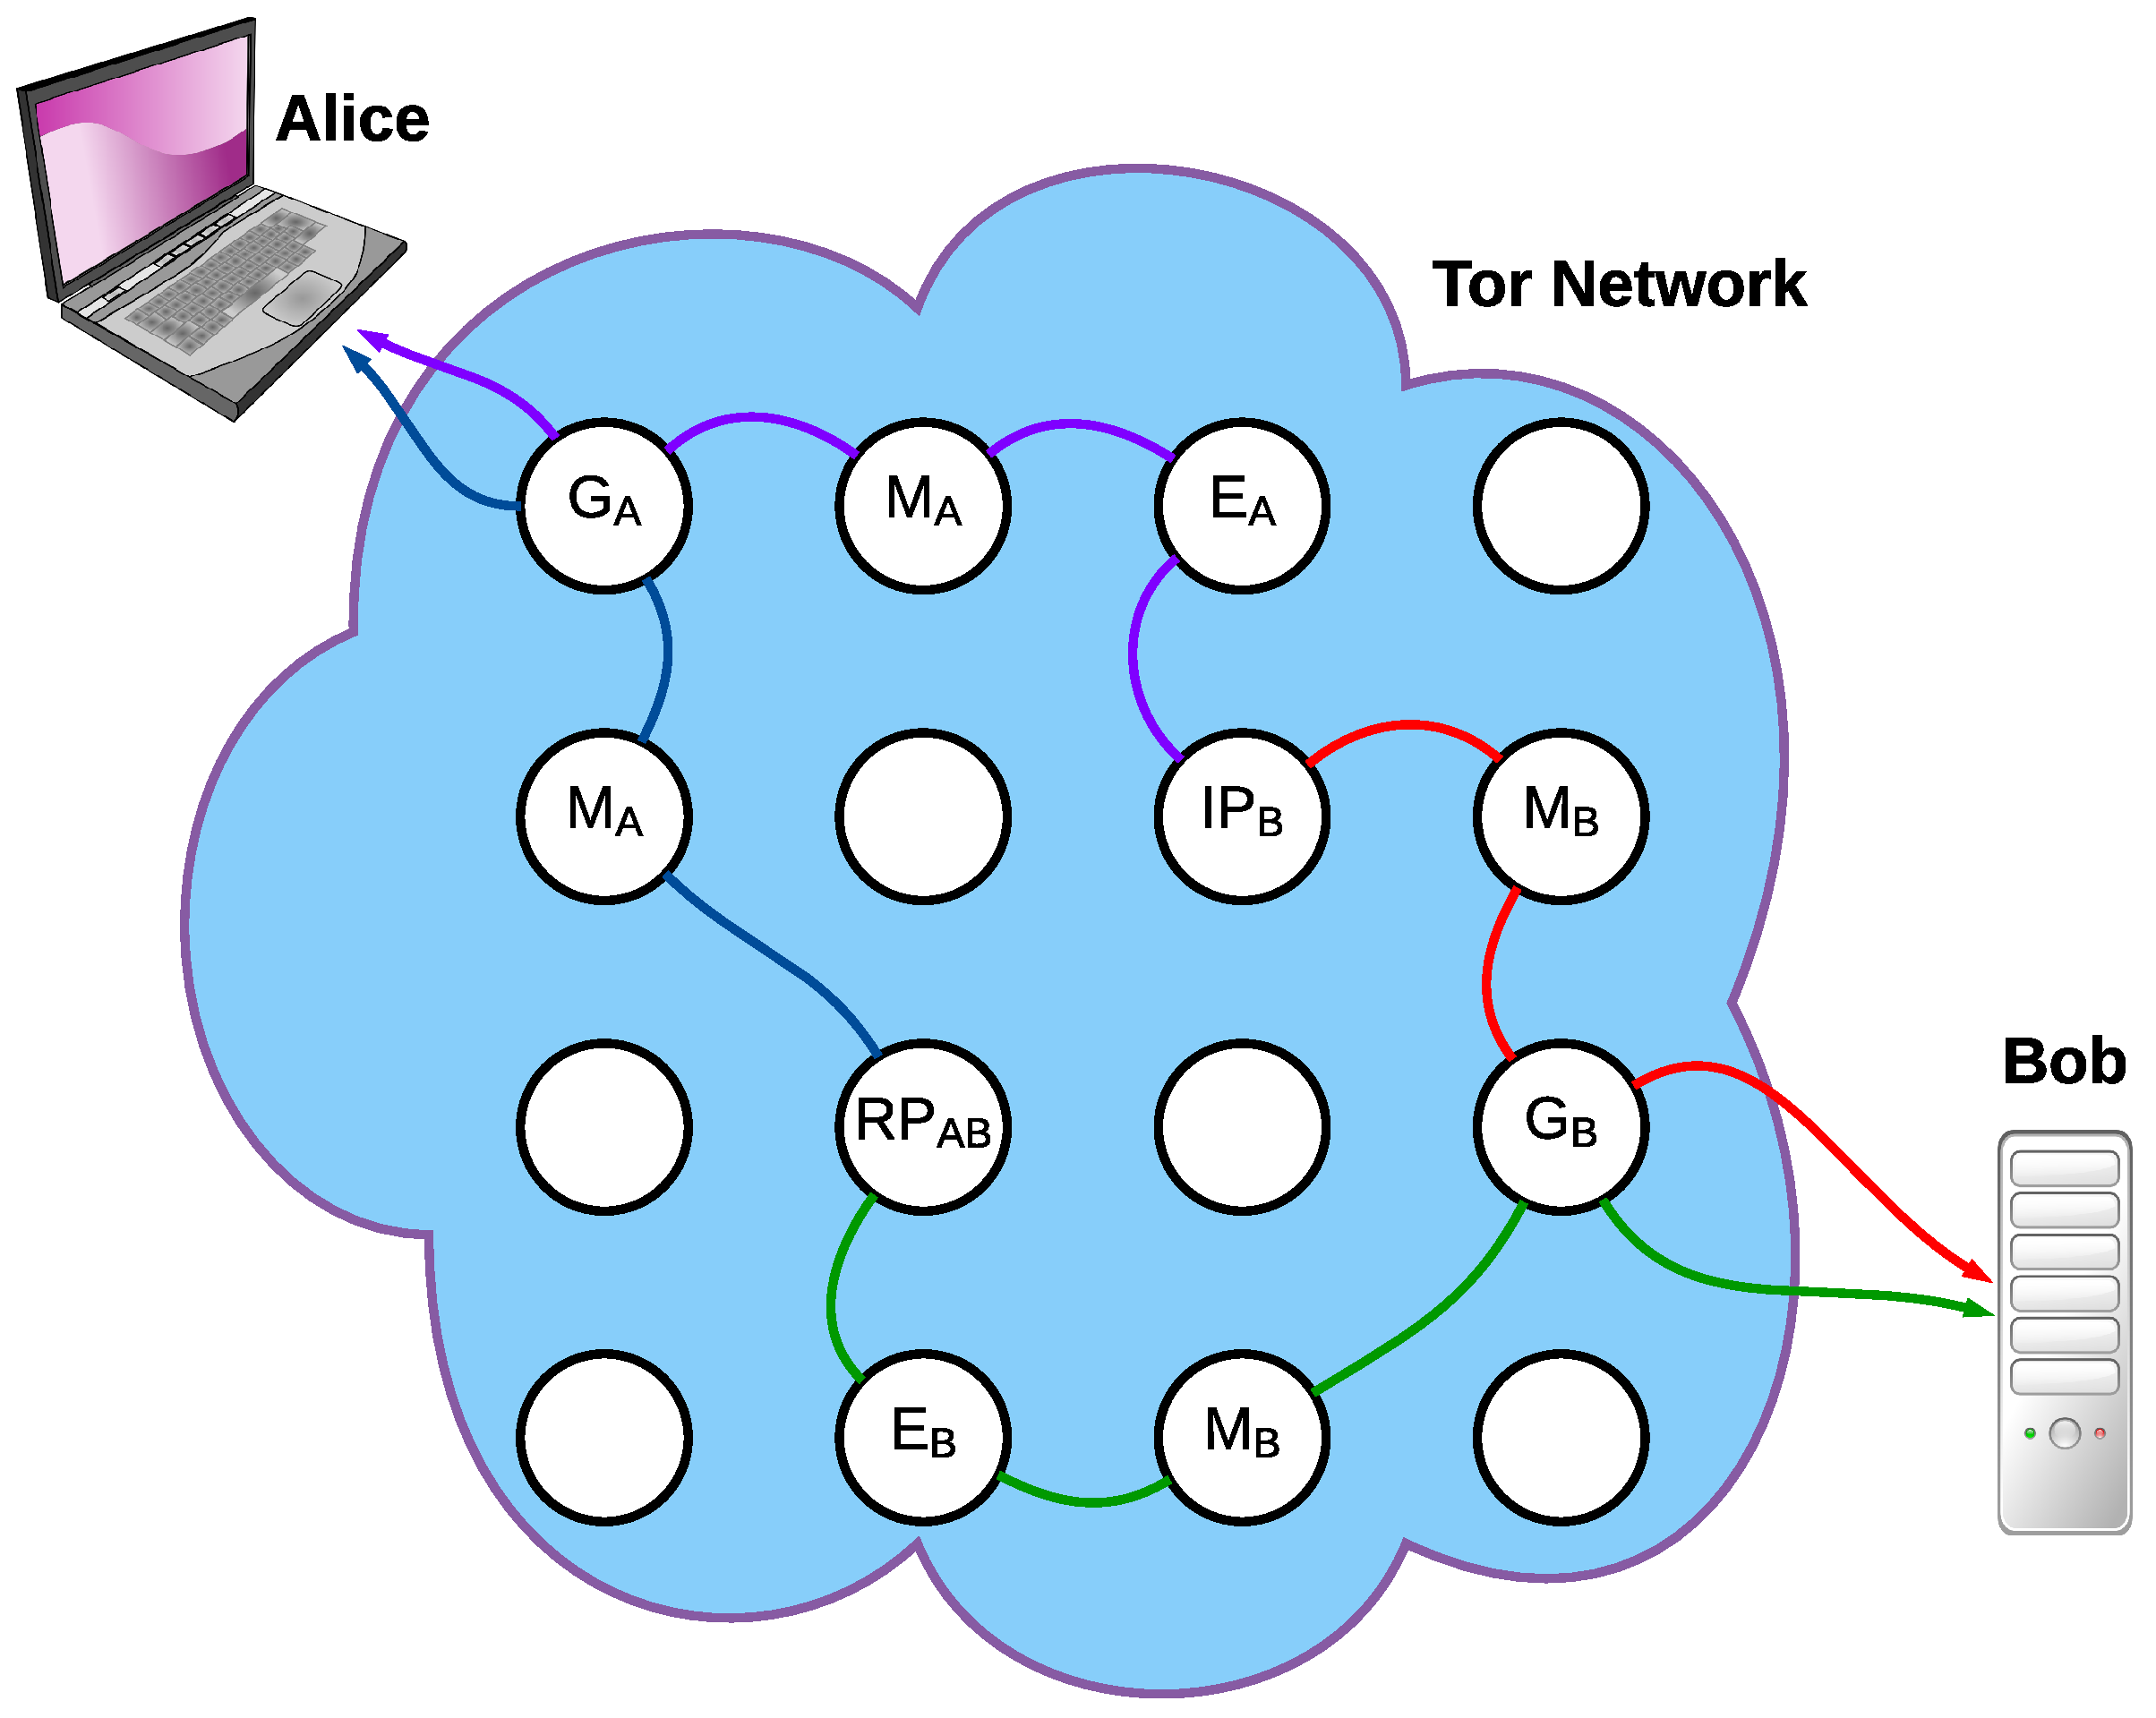
\includegraphics[width=0.9\linewidth]{../assets/images/LucidCharts/Hidden_Services.pdf}
	\caption{A Tor client, Alice, and a hidden service, Bob, first mate two Tor circuits (purple and red) at one of Bob's long-term \emph{introduction points} (IP). They then renegotiate and communicate over another pair of Tor circuits (blue and green) at an ephemeral \emph{rendezvous point} (RP). This achieves communication with bi-directional anonymity \cite{overlier2006locating}.}
\end{figure}

Tor hidden service addresses are distributed and globally collision-free, but there is a strong discontinuity between the address and the service's purpose. As their addresses usually contain no human-readable information, a visitor cannot categorize, label, or authenticate hidden services in advance. While a Tor user may explore and bookmark hidden services within the Tor Browser, this is a very narrow solution and does not scale well past a few dozen bookmarks. Over time, third-party directories -- both on the clearnet and darknet -- have appeared in an attempt to counteract this issue, but these directories must be constantly maintained and the approach is neither convenient nor does it practically scale past several hundred entries. The approximately 27,000 hidden services currently on the Tor network (Figure \ref{fig:OnionCount}) and the potential for continued growth both suggest the strong need for a more complete and wider solution to solve the usability issue.

\begin{figure}[htbp]
	\centering
	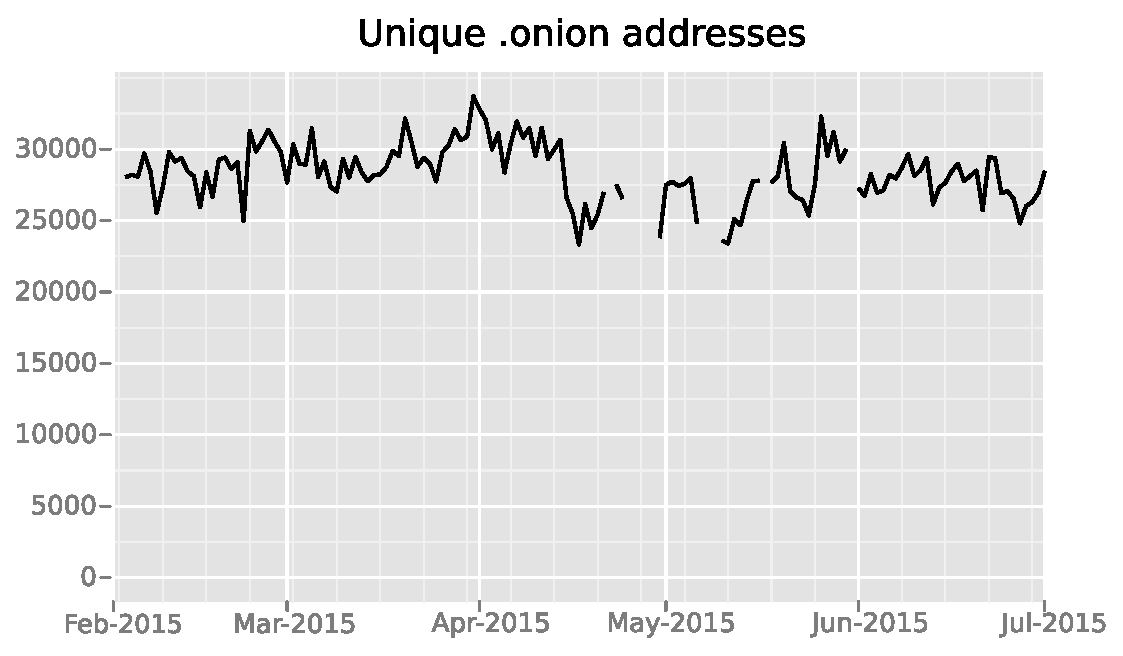
\includegraphics[width=\linewidth]{../assets/images/Tor/onion_2015-02_2015-07.eps}
	\caption{The number of unique .onion addresses seen in the Tor network between February 2015 and July 2015 \cite{kadianakis2015extrapolating}\cite{TorMetrics}.}
	\label{fig:OnionCount}
\end{figure}

\subsection{Contributions}

In this paper, we present the design, analysis, and implementation of the Onion Name System, (OnioNS) a distributed, secure, and usable domain name system for Tor hidden services. Any hidden service can claim a meaningful human-readable domain name without loss of anonymity and clients can query against OnioNS in privacy-enhanced and verifiable manner. OnioNS is powered by a random subset of nodes within the existing Tor network, significantly limiting the additional attack surface. We devise a distributed database that is resistant to node compromise and provides authenticated denial-of-existence. We provide a backwards-compatible plugin for the Tor Browser and demonstrates the high usability and performance of OnioNS. To the best of our knowledge, this is the first alternative DNS for Tor hidden services which is distributed, secure, and usable at the same time.

\textbf{Paper Organization:} This paper is divided into four main sections. In section \ref{sec:problemStatement} we define our design objectives and explain why existing works do not meet our goals. We also define our threat model, which includes Tor's assumptions and the capabilities of our adversaries. In section \ref{sec:Solution}, we describe the system overview and define several key protocols. In section \ref{sec:Analysis} we analyse the security of our assumptions and examine other attack vectors. Last, in section \ref{sec:Evaluation} we describe our implementation prototype, perform performance analysis tests, and demonstrate that our software allows the Tor Browser to load a hidden service under a meaningful domain name.

\section{Problem Statement}
\label{sec:problemStatement}

To integrate with Tor, we must provide a secure system, preserve user privacy, and avoid compromising other areas of the Tor network. Additionally, we seek to achieve all three properties of Zooko's Triangle (section \ref{sec:ZookosTriangle}) and to providing a mechanism for authenticated denial-of-existence (section \ref{sec:authDenialIntro}).

\subsection{Design Objectives}

Tor's privacy-enhanced environment introduces distinct challenges to any new infrastructure. Here we enumerate a list of requirements that must be met by any naming system applicable to Tor hidden services. In Section \ref{sec:RelatedWorks} we analyse existing works and show how these systems do not meet these goals and in Section \ref{sec:Solution} we demonstrate how we overcome them with OnioNS.

1. \textbf{Anonymous registrations}: The system should not require any personally-identifiable or location information from the registrant. Tor hidden services publicize no more information than a public key and a set of Introduction Points.

2. \textbf{Privacy-enhanced queries}: Clients should be anonymous, indistinguishable, and unable to be tracked by name servers. Tor already tunnels most Internet DNS queries over circuits, thus any alternative naming system should continue to preserve user privacy during lookups.

3. \textbf{Strong integrity}: Clients must be able to verify that the domain-address pairing that they receive from name servers is authentic relative to the authenticity of the hidden service. This objective provides a defence against phishing attacks.

4. \textbf{Globally unique domain names}: Any domain name of global scope must point to at most one server. For naming systems that generate names via cryptographic hashes, the key-space must be of sufficient length to resist cryptanalytic attack. Unique domain names prevent fragmentation of users and also provides a defence against phishing attacks.

5. \textbf{Distributed control}: Central authorities carry absolute control over the system and root security breaches can easily compromise the integrity of the entire system. They may also be able to compromise the privacy of both users and hidden services or may not allow anonymous registrations.

6. \textbf{High usability}: Most Tor users are not security experts or have technical backgrounds. The system must resolve protocols with minimal input from the user and hide non-essential details.

7. \textbf{Optional}: Not all hidden services require meaningful names. For example, applications such as Ricochet \cite{RicochetGithub} may create ephemeral hidden services where names may not be appropriate or necessary. Thus a naming system should be optional but not required. Systems that provide backwards compatibility by preserving the Tor hidden service protocol also achieve this property.

8. \textbf{Lightweight}: In most realistic environments clients have neither the bandwidth nor storage capacity to hold the system's entire database, nor the capability of meeting significant computation burdens. The system should have a minimal impact on Tor clients and hidden services.

\subsection{Challenges}

\subsubsection{Zooko's Triangle}
\label{sec:ZookosTriangle}

In 2001, Zooko Wilcox-O'Hearn described three desirable properties for any persistent naming system: distributed design, assignment of human-meaningful names, and globally unique names. In a statement now known as Zooko's Triangle, \cite{ferdous2009security}\cite{stiegler2005petname} he claimed any naming system could only achieve two of these properties. This is illustrated in Figure \ref{fig:ZookosTriangle}.

\begin{figure}[htbp]
	\centering
	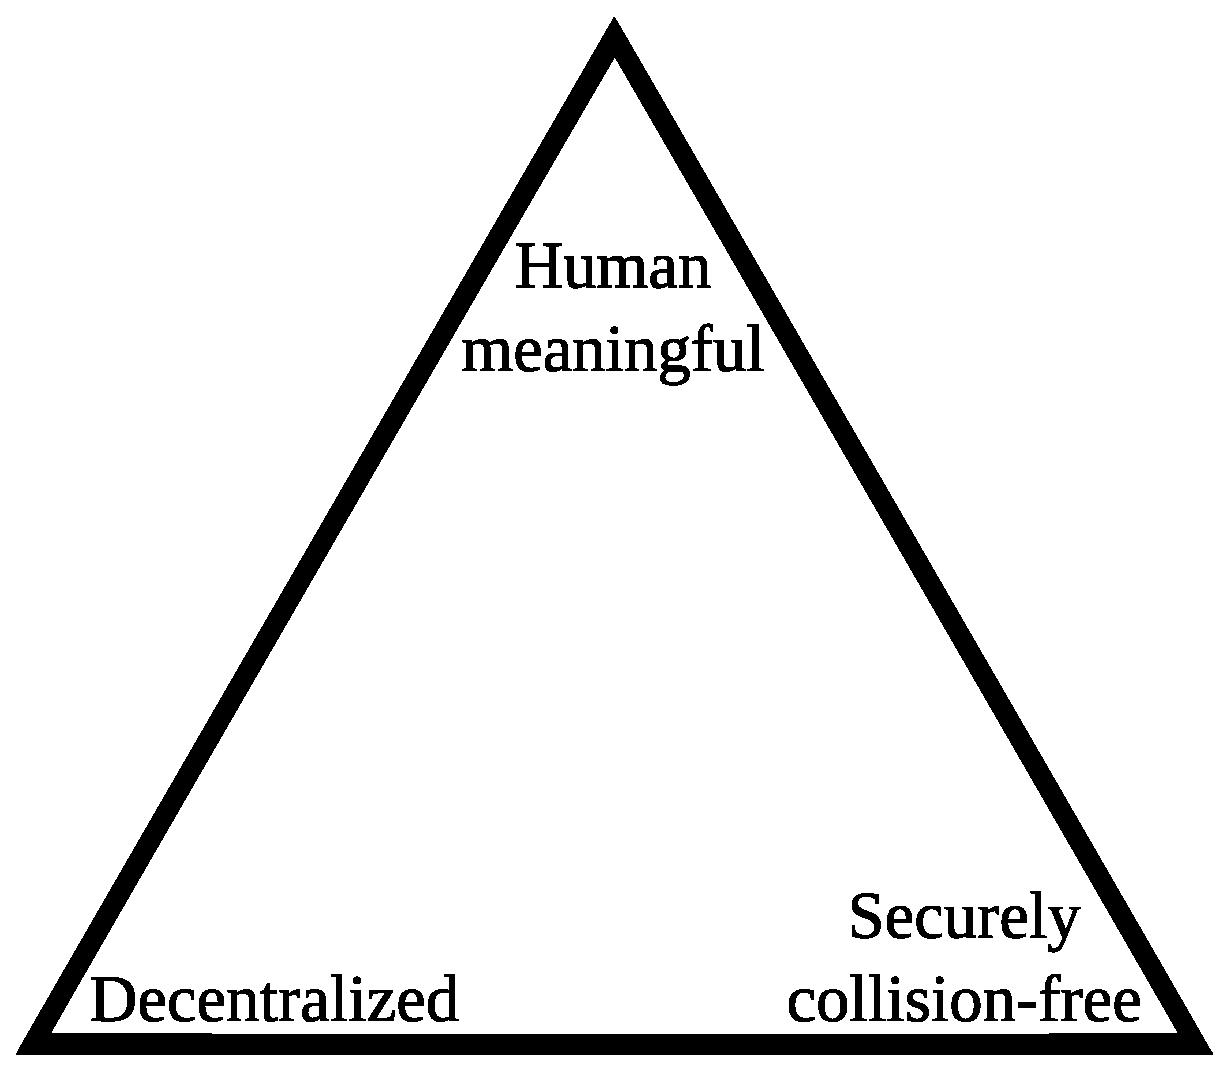
\includegraphics[width=0.3\textwidth]{../assets/images/Zooko.eps}
	\caption{Zooko's Triangle.}
	\label{fig:ZookosTriangle}
\end{figure}

Some examples of naming systems that achieve only two of these properties include:

\begin{itemize}
	\item \textbf{Securely unique and human-meaningful} \\ --- Internet domain names.
	\item \textbf{Decentralized and human-meaningful} \\ --- Human names and nicknames.
	\item \textbf{Securely unique and decentralized} \\ --- PGP keys and Tor .onion addresses.
\end{itemize}

\subsubsection{Authenticated Denial-of-Existence}
\label{sec:authDenialIntro}

When a client queries a name server for a name, the server may respond in three distinct ways:

\begin{enumerate}
	\item It may return the correct destination.
	\item It may return a spoofed destination.
	\item It may claim that an existing name does not exist.
	\item It may choose not to answer.
\end{enumerate}

Cases two and three may be expected by a malicious name server and constitute significant threats to the client. On the Internet, the second case is addressed with SSL certificates and a chain of trust to root Certificate Authorities (CAs) but the third case is not addressed by DNS and remains a possible attack vector. DNSSEC includes an extension for Hashed Authenticated Denial of Existence (NSEC3) which provides signed non-existence claims on a per-domain basis. However, DNSSEC has not seen widespread use, storing per-domain denial-of-existence records introduces significant storage requirements, and to our knowledge no alternative DNS provides mechanisms for authenticated denial-of-existence. Closing this attack vector is not easy; the na\"{i}ve solution of generating proof individually or en-masse for every non-existent domain is infeasible since the domain space is likely too large to practically enumerate.

\section{Related Works}
\label{sec:RelatedWorks}

Vanity key generators (e.g. Shallot \cite{KatmagicShallot}) attempt to find by brute-force an RSA key that generates a partially-desirable hash. Vanity key generators are commonly used by hidden service operators to improve the recognition of their hidden service, particularly for higher-profile services \cite{syversongenuine}. For example, a hidden service operator may wish to start his service's address with a meaningful noun so that others may more easily recognize it. However, these generators are only partially successful at enhancing readability because the size of the domain key-space is too large to be fully brute-forced in any reasonable length of time. If the address key-space was reduced to allow a full brute-force, the system would fail to be guaranteed collision-free. Nicolussi suggested changing the address encoding to a delimited series of words, using a dictionary known in advance by all parties \cite{nicolussi2011human}. While Nicolussi's encoding improves the readability of an address, like vanity key generators it does not allow addresses to be completely meaningful.

The Internet DNS is already well established as a fundamental abstraction layer for Internet routing. However, despite its widespread use and extreme popularity, the Internet DNS suffers from several significant shortcomings and fundamental security issues that make it inappropriate for use by Tor hidden services. Generally speaking, the Internet DNS by default does not use any cryptographic primitives. DNSSEC is primarily designed to prevent forgeries and DNS cache poisoning from intermediary name servers and it does not provide any degree of query privacy \cite{wachs2014censorship}. Additional extensions and protocols such as DNSCurve \cite{bernstein2009dnscurve} have been proposed, but DNSSEC and DNSCurve have not yet seen widespread full deployment across the Internet. Cachin and Samar \cite{cachin2004secure} extended the Internet DNS and decreased the attack potential for authoritative name servers via threshold cryptography, but the lack of default security in the Internet DNS and the logistical difficulty in globally implementing their work prevents us from using their system for hidden services.

Scaife et al. created OnionDNS \cite{Scaife2015oniondns}, a seizure-resistant alternative resolution service for the Internet. OnionDNS is based on DNS and uses unmodified BIND client software but anonymizes the root server by hosting it as a hidden service. While OnionDNS is highly usable and provides DNSSEC and other authentication mechanisms, the system is centralized by a single root server and thus highly vulnerable if the root is malicious or is compromised.

The GNU Name System \cite{wachs2014censorship} (GNS) is a decentralized alternative DNS. GNS distributes names across a hierarchical system of zones constructed into directed graphs. Each user manages their own zone and distributes zone access peer-to-peer within social circles. However, GNS does not guarantee that names are \emph{globally} unique. Furthermore, the selection of a trustworthy zone to use would be a significant challenge for using GNS for Tor hidden services and such a selection no longer makes the system distributed. Awerbuch and Scheideler, \cite{awerbuch2004group} constructed a distributed peer-to-peer naming system, but like GNS, made no guarantee that domain names would be globally unique.

Namecoin \cite{NamecoinHome} is an early fork of Bitcoin \cite{nakamoto2008bitcoin} and is noteworthy for achieving all three properties of Zooko's Triangle. Namecoin holds information transactions in a distributed ledger known as a blockchain. Transactions and information are added to the head of the blockchain by ``miners,'' who solve a proof-of-work problem to generate the next block. While Namecoin is often advertised as capable of assigning names to Tor hidden services, it has several practical issues that make it generally infeasible to be used for that purpose. First, Namecoin does not provide a mechanism for proving ownership of domain names; this makes it difficult for a client to prove that the owner of the hidden service private RSA key also maintains the Namecoin secp256k1 ECDSA private key. Second, Namecoin generally requires users to pre-fetch the blockchain which introduces significant logistical issues due to high bandwidth, storage, and CPU load. Third, although Namecoin supports anonymous ownership of information, it is non-trivial to anonymously purchase Namecoins, thus preventing domain registration from being truly anonymous. These issues prevent Namecoin from being a practical alternative DNS for Tor hidden services.

% todo: explain why the SPV or whatever clients don't work, or include OnionDNS's criticisms. This might not be necessary.

\section{Assumptions and Threat Model}
\label{sec:threatModel}

We assume that Tor circuits provides privacy and anonymity; if Alice constructs a three-hop Tor circuit to Bob with modern Tor cryptographic protocols and sends a message $ m $ to Bob, we assume that Bob can learn no more about Alice than the contents of $ m $. This implies that if $ m $ does not contain identifiable information, Alice is anonymous from Bob's perspective. This also implies an assumption on the security of cryptographic primitives and a lack of backdoors or analogous breaks in cryptographic libraries. The security of Tor circuits is also dependent on the honesty of directory authorities: we also assume that more than fifty percent of Tor directory authorities are at least semi-honest; they may wiretap but are not capable of violating protocols. The aforementioned assumptions are shared by the Tor network.

We assume that Eve controls some percentage of dishonest colluding Tor routers as well as semi-honest routers, however this percentage is small enough to avoid violating our second assumption. We assume a fixed percentage of dishonest and semi-honest routers; namely that the percentage of routers under an Eve's control does not increase in response to the inclusion of OnionNS into Tor infrastructure. This assumption simplifies our threat model analysis but we consider it realistic because while Tor traffic is purposely secret as it travels through the network, we consider OnioNS information public so we don't consider the inclusion of OnioNS a motivating factor to Eve.

% todo: this paragraph is now out-of-date
Let $ R $ be the set of Tor routers with the Fast, Stable, and Running flags and let $ Q $ be an $ M $-sized set randomly chosen from $ R $ with selection probability $ P (Q_{i}) = \frac{Q_{i}(w)}{\sum_{j=0}^{\| R \|} R_{j}(w)} $ where $ Q_{i}(w) $ is $ Q_{i} $'s consensus weight as determined by Tor directory authorities. We then assume that $ Q $ is under the influence of zero or more adversaries and that largest subset of agreeing routers in $ Q $ are at least semi-honest.

We assume no upper-bound on the computational capabilities of any adversary, with the exception that they are unable to compromise cryptographic primitives. However, we assume that the adversary has a fixed budget, namely that they have a quota on the memory and CPU hours that they can allocate against our system. We further assume that an adversary may try to gain control of authoritative OnioNS servers through a Sybil attack on the Tor network or that they may operate any of the non-authoritative name servers

\subsection{Use Cases}
\label{sec:useCases}

As hidden services require no more than a configured Tor client and a socket listener and are thus cheap to create, we anticipate that actors in our system will perform any of the following use cases:

\begin{enumerate}
	\item \textbf{Create many hidden services to register many names.}
	\item \textbf{Create one hidden service to register many names.}
	\item \textbf{Create many hidden services to register a single name.}
	\item \textbf{Create one hidden service to register a single name.}
\end{enumerate}

Sceneries one and two are expected to be performed by adversaries attempting to register all popular names in a ``land rush'' for financial gain or as a denial-of-registration attack. Scenario three may indicate an attempt by many legitimate actors to claim a highly desirable name, while scenario four is the expected behaviour of innocent actors. As hidden services are anonymous by nature, it is not straightforward to construct a system that differentiates and selects between a single actor performing the first scenario and many actors performing the fourth scenario. However, as well-known hidden services cannot change their public key, we expect innocent actors to follow the fourth use case.

\section{Solution}
\label{sec:Solution}

\subsection{Cryptographic Primitives}
\label{sec:cryptoPrimitives}

OnioNS utilizes hash functions, digital signature algorithms, a proof-of-work scheme, and a global source of randomness.

\begin{itemize}
	\item Let $ \mathcal{H}(x) $ be a cryptographic hash function. In our reference implementation we define $ \mathcal{H}(x) $ as SHA-384.
	\item Let $ S_{\mathit{RSA}}(m, r) $ be a deterministic RSA digital signature function that accepts a message $ m $ and a private RSA key $ r $ and returns a digital signature. Let $ S_{\mathit{RSA}}(m, r) $ use $ \mathcal{H}(x) $ as a digest function on $ m $ in all use cases. In our reference implementation we define $ S_{\mathit{RSA}}(m, r) $ as EMSA PKCS1 v1.5. (EMSA3)
	\item Let $ V_{\mathit{RSA}}(m, R) $ validate an RSA digital signature by accepting a message $ m $ and a public key $ R $, and return true if and only if the signature is valid.
	\item Let $ \mathrm{PoW}(k) $ be a one-way function that accepts an input key $ k $ and returns a deterministic output. Our reference implementation uses the scrypt \cite{percival2012scrypt} key derivation function with a fixed salt.
	\item Let $ \mathcal{G}(t) $ be a cryptographically-secure generator of random or pseudorandom timestapped numbers. $ \mathcal{G}(t) $ deterministically returns a value for time $ t $ in the present or past.
	\item Let $ \mathcal{R}(s) $ be a pseudorandom number generator that accepts an initial seed $ s $ and returns a list of pseudorandom numbers. In our design, $ s = \mathcal{G}(t) $, so $ \mathcal{R}(s) $ does not need to be cryptographically secure. We suggest MT19937, commonly known as the Mersenne Twister. This generator is widely used throughout most programming languages and is well known for its speed, long period, and the high quality of its pseudorandom output \cite{matsumoto1998mersenne}.
\end{itemize}

\subsection{Definitions}

\textbf{domain name} The syntax of OnioNS domain names mirrors the Internet DNS; we use a sequence of name-delimiter pairs with a .tor pseudo-TLD. The Internet DNS defines a hierarchy of administrative realms that are closely tied to the depth of each name. By contrast, OnioNS makes no such distinction; we let hidden service operators claim second-level names and then control all names of greater depth under that second-level name.

%todo: define this as a ticket or a post-lottery record
A \textbf{ticket} contains $ \mathit{type} $, the purpose of this structure; $ \mathit{name} $, a meaningful second-level domain name with the .tor pseudo-TLD; $ \mathit{subdomains} $, a one-to-one map of .tor domains of level three or higher to .tor or .onion destinations; $ \mathit{contact} $, an optional PGP fingerprint; $ \mathit{rand} $, the output of $ \mathcal{G}(i) $ (section \ref{sec:rngProcess}); $ \mathit{nonce} $, bytes used as a variable for the proof-of-work; $ \mathit{pow} $, the output of $ \mathrm{PoW}(i) $; $ \mathit{signature} $, the output of $ S_{\mathit{RSA}}(m, r) $; and $ \mathit{pubHSKey} $, Bob's public RSA key. If $ \mathit{type} $ is set to any of the operations described in section \ref{sec:recordOps}, this data structure is known as a \textbf{record}.

A \textbf{mirror} is Tor router that is acting as a name server within the OnioNS network. Mirrors maintain a textual database of system information and respond to client queries but usually do not accept new DNS records or other information from hidden services. We note that mirrors may be outside the Tor network, but this scenario is outside the scope of this work.

\textbf{Quorum candidates} are mirrors that provide proof in Tor's consensus documents that they hold a current copy of the database and that they have sufficient CPU and bandwidth capabilities to handle OnioNS communication in addition to their normal Tor duties.

The \textbf{Quorum} is authoritative subset of Quorum candidates who have active responsibility over the OnioNS database. Quorum nodes accept and process information from hidden services but do not respond to client queries. The Quorum is randomly chosen from the set of Quorum candidates and is rotated periodically, as described in section \ref{sec:protocols}.

\renewcommand{\arraystretch}{1.2}
\begin{table}[h]
	\small
	\begin{tabularx}{\linewidth}{ | l | X | }
		\hline
    	$ L_{Q} $ & the size of the Quorum \\ \hline
    	$ L_{T} $ & the number of routers in the Tor network \\ \hline
    	$ Q_{i} $ & the $ i $th Quorum where $ i $ is an iteration counter \\ \hline
    	$ \Delta q $ & the lifetime of a Quorum in days \\ \hline
  	\end{tabularx}
  	\vspace{6pt}
  	\caption{Frequently used notations}
\end{table}

\subsection{Infrastructure}

%\begin{figure}[htbp]
%	\centering
%	\begin{tikzpicture}[scale=0.74, ->, node distance=2.5cm, main node/.style={circle, fill=blue!20, draw, font=\sffamily\bfseries, transform shape}]
%
%			\node[main node] (1) {$ A_{G} $};
%			\node[main node] (2) [right of=1] {};
%			\node[main node] (3) [right of=2] {Alice};
%			\node[main node] (4) [right of=3] {};
%
%			\node[main node] (5) [below of=1] {$ A_{E} $};
%			\node[main node] (6) [right of=5] {$ A_{M} $};
%			\node[main node] (7) [right of=6] {};
%			\node[main node] (8) [right of=7] {};
%
%			\node[main node] (9) [below of=5] {};
%			\node[main node] (10) [right of=9] {OnioNS};
%			\node[main node] (11) [right of=10] {};
%			\node[main node] (12) [right of=11] {$ B_{E} $};
%
%			\node[main node] (13) [below of=9] {};
%			\node[main node] (14) [right of=13] {$ B_{M} $};
%			\node[main node] (15) [right of=14] {$ B_{G} $};
%			\node[main node] (16) [right of=15] {Bob};
%
%			% Alice-OnioNS conversation
%			\tikzstyle{EdgeStyle}=[bend right, -, green]
%			\Edge[](3)(1)
%			\tikzstyle{EdgeStyle}=[bend left=15, -, green]
%			\Edge[](1)(6)
%			\Edge[](5)(6)
%			\draw[thick, ->, red, postaction={decorate, decoration={text along path, text align=center, text={query}, raise=4pt}}] (5) to [bend left=10] (10){};
%			\draw[thick, <-, blue, postaction={decorate, decoration={text along path, text align=center, text={response}, raise=-9pt}}] (5) to [bend right=10] (10){};
%
%			% Bob-OnioNS conversation
%			\tikzstyle{EdgeStyle}=[bend right=15, -, green]
%			\Edge[](16)(15)
%			\Edge[](15)(14)
%			\tikzstyle{EdgeStyle}=[bend left=12, -, green]
%			\Edge[](14)(12)
%			\draw[thick, red, <-, postaction={decorate, decoration={text along path, text align=center, text={record}, raise=3pt}}] (10) to [bend left=40] (12){};
%			\draw[thick, blue, ->, postaction={decorate, decoration={text along path, text align=center, text={confirmation}, raise=-10pt}}] (10) to [bend left=30] (12){};
%
%		\end{tikzpicture}
%	\caption{Bob uses a Tor circuit ($ B_{G} $, $ B_{M} $, $ B_{E} $) to anonymously broadcast a record to OnioNS. Alice uses her own Tor circuit ($ A_{G} $, $ A_{M} $, $ A_{E} $) to query the system for a domain name, and she is given Bob's record in response. Then Alice connects to Bob by Tor's hidden service protocol.}
%	\label{fig:basicDesign}
%\end{figure}

We embed OnioNS infrastructure within the Tor network by utilizing existing Tor nodes as hosts for OnioNS mirrors. Each Tor node may opt to run a hidden services which then powers a OnioNS mirror running on localhost. As these hidden services are part of OnioNS, they must be accessed by their traditional .onion address, but this is acceptable as these servers are never accessed directly by end-users. Our reliance on hidden services allows us to recycle existing TLS links between Tor nodes and leverage Tor circuits to obscure all communication between end-users and OnioNS infrastructure without requiring a modification to the Tor executable. In essence, all communication with or within OnioNS is hidden from outside observers by ephemeral internal Tor circuits that need not pass through exit routers, increasing privacy and reducing our attack surface.

We authenticate servers in our infrastructure using Ed25519 \cite{bernstein2011high} keys; as of Tor 0.2.7, Tor routers generate and manage Ed25519 keypairs and include their public key in the network consensus. We use Ed25519 because of its strength, size, and speed advantages over Tor's original RSA-1024 identity keys. OnioNS servers provide proof-of-knowledge of their private Ed25519 key for all outbound traffic on their hidden service, achieving end-to-end authentication of all OnioNS communication. Throughout the remainder of this paper, ``hidden services'' refers exclusively to hidden services that are not part of the OnioNS infrastructure.

Each mirror maintains two distinct databases; ``main'' and ``ephemeral'', which both contain records. Newly received records are temporarily stored in the ephemeral database, which is periodically merged into the main database. Mirrors use their main database to respond to clients, who can then authenticate the responses against information published by Quorum nodes. Quorum nodes maintain an additional and secret database that contains lottery tickets.


%Mirrors return records from this database to clients, who can then use the published state to authenticate the mirror's responses, as described in section \ref{sec:authDenial}. 
% Twelve hours prior to the rotation of the Quorum, mirrors merge the ephemeral database into the authenticated database and publish the new state of the authenticated database in the network consensus, as described in section \ref{sec:qQualification}.



%\begin{figure}[h]
%	\centering
%	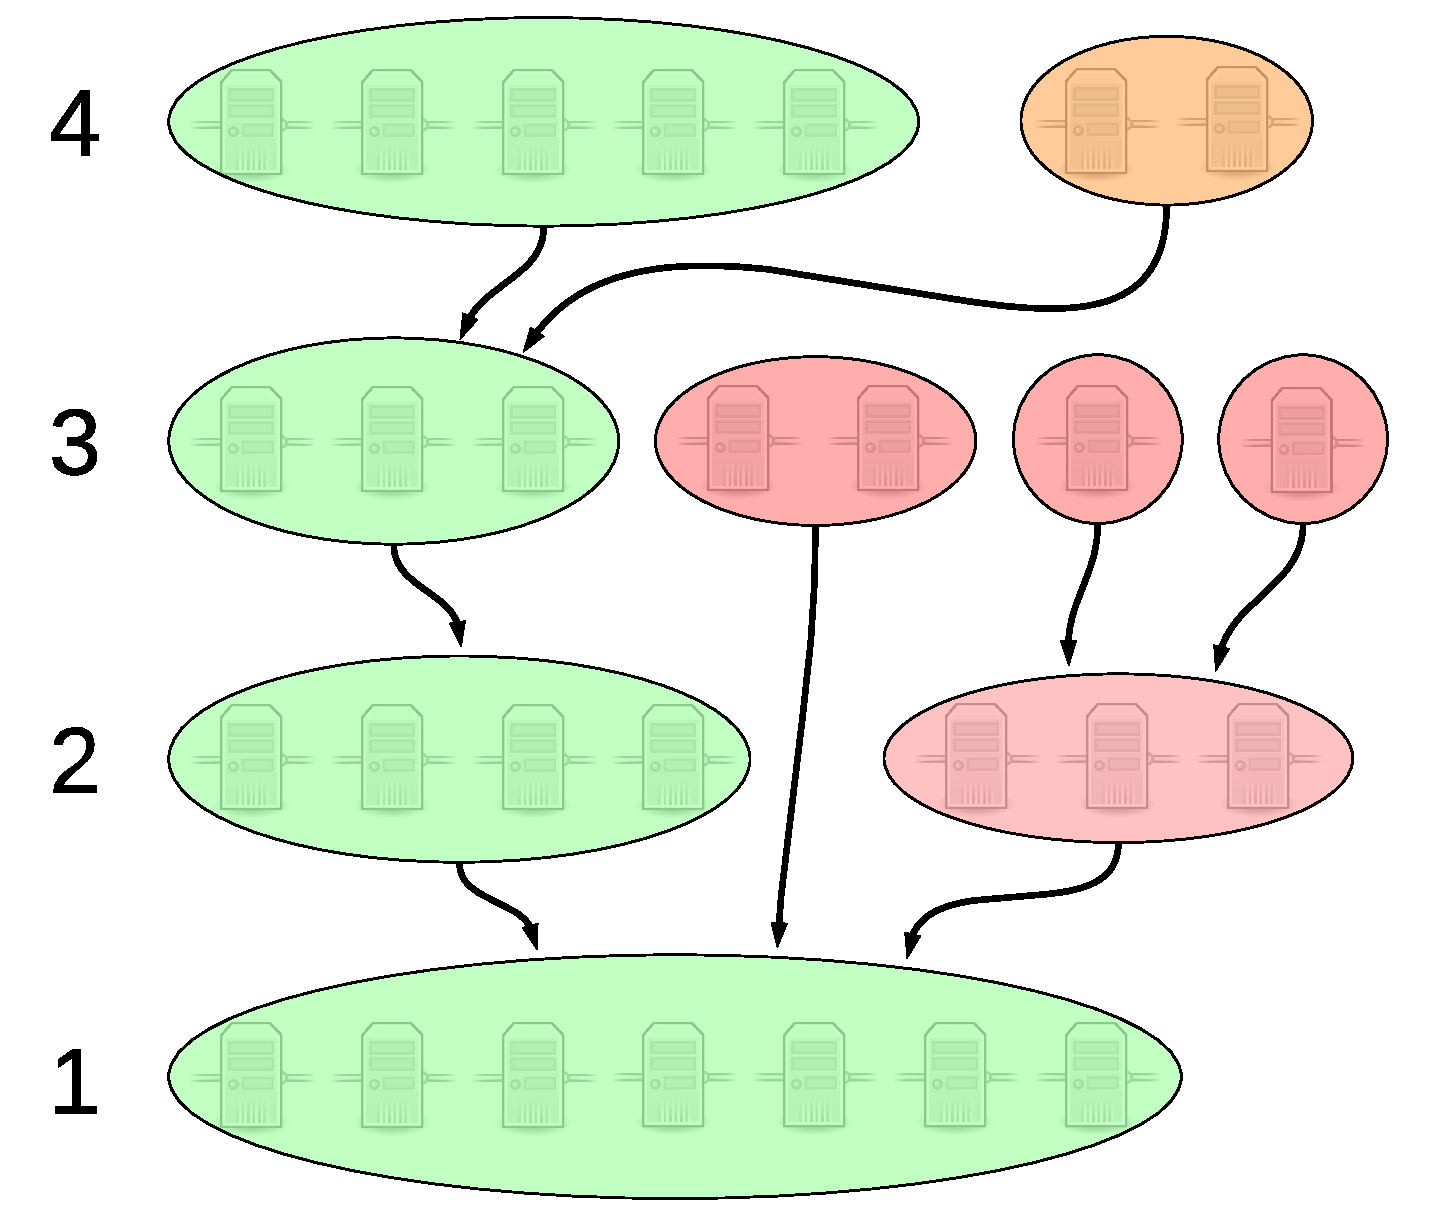
\includegraphics[width=0.4\linewidth]{../assets/images/LucidCharts/Page-chain2.pdf}
%	\caption{THIS IS A PLACEHOLDER IMAGE. TODO: create picture illustrating the complete Quorum graph + mirrors subscribing. A high-level overview of OnioNS infrastructure running within the Tor network. Green links indicate client-to-HS connections. Hidden service operators send requests for names and records directly to Quorum nodes, while clients use mirrors as name servers.}
%	\label{fig:lotteryTimeline}
%\end{figure}



%nuance: repeated information is not replayed
% some Q members could be malicious, how are subscriptions handled?

% mention Merkle tree?
% overview of protocols and database management?


\subsection{Protocols}
\label{sec:protocols}

We now describe the protocols fundamental to OnioNS functionality. These protocols are listed according to their approximate order of execution in OnioNS.

% provide timeline or summary here?

\subsubsection{Random Number Generation} % done
\label{sec:rngProcess}

We use $ \mathcal{G}(t) $ as a basis for several of our protocols, although we note that $ \mathcal{G}(t) $ has applications in Tor beyond OnioNS. One straightforward definition of $ \mathcal{G}(t) $ is the SHA-384 hash of Tor's consensus documents. If the Tor network is dynamic enough to provide significant amounts of entropy into the consensus documents, then $ \mathcal{G}(t) $ may be considered cryptographically secure. However, this assumption does not hold because current router descriptors are publicly available before the consensus documents are published, allowing $ \mathcal{G}(t) $ under this approach to be easily manipulated by a few malicious Tor routers. The attack becomes significantly easier in the final moments before the directory authorities publish the consensus.

Instead, we suggest implementing $ \mathcal{G}(t) $ as the commitment scheme proposed by Goulet and Kadianakis \cite{GouletCommitReveal}. Their algorithm modifies the consensus voting protocol that is run once an hour by Tor directory authorities. In their scheme, at 00:00 UTC each authority commits a SHA-256 hash of a secret value $ x $ into each consensus vote across a 12 hour period. Then at 12:00 UTC, each directory authority reveals $ x $ across the next set of 12 consensuses. Then at 24:00 UTC, the revealed values are hashed together to create a single random number, which is then embedded in the consensus documents so that it is efficiently distributed to both Tor routers and clients. A different random number thus appears in the consensus every 24 hours. While this implementation of $ \mathcal{G}(t) $ defines $ t $ as an integer of 24 hours, $ \Delta q $ may be greater than 24 hours, as discussed in \ref{sec:qRotation}. Therefore, throughout the remainder of this document we will use the notation $ \mathcal{G}(i) $ to reference the $ \mathcal{G}(t \dot 24 \dot \Delta q) $ that defines $ Q_{i} $.

%todo: need image here to explain the cycle and Quorum lifetime

The two time boundaries in this implementation of $ \mathcal{G}(t) $ trigger events within our system. The publication of $ \mathcal{G}(i) $ at midnight defines the selection of the next Quorum, causes all mirrors to publish the state of their database, marks the beginning of the next lottery, and determines the winners of the previous lottery. The first reveal at 12:00 UTC ends the lottery and contains the pool of Quorum candidates. We clarify our distinction of these boundaries in section \ref{sec:RandGeneration}. 

% todo: verify that these timings are reflected in the below protocols

\subsubsection{Quorum Qualification} % done
\label{sec:qQualification}

Quorum candidates must prove that they are both up-to-date mirrors and that they have sufficient capabilities to handle the increased communication and processing demands from OnioNS protocols, an additional burden on top of their traditional Tor responsibilities.

The na\"{i}ve solution to demonstrating the first requirement is for all participants to simply ask mirrors for their internal database, and then compare the recency of its database against the databases from the other mirrors. However, this solution does not scale well; Tor has $ \approx $ 2.1 million daily users \cite{TorMetrics}: it is infeasible for any single node to handle queries from all of them. Instead, at 00:00 UTC each day, let each mirror merge the ephemeral database into the main database, recompute the Merkle tree described in section \ref{sec:authDenial}, and place the root hash inside the Contact field of its router descriptor so that the hash appears in the network consensus. The Contact field is typically used to hold the email address and PGP fingerprint of the router's administrator, but our use of the Contact field allows us to distribute the hash without modifying Tor infrastructure. Mirrors should also distribute their hidden service address in the same way. %These values could also be held in new descriptor fields, which we will explore after publication.

Tor provides a mechanism for demonstrating the latter requirement; Quorum candidates must have the Fast, Stable, and Running flags. Tor routers with higher CPU or bandwidth capabilities relative to their peers also receive a proportionally larger consensus weight from the directory authorities. This consensus weight in turn strongly influences router selection during circuit construction: routers with higher weights are more likely to be chosen in a circuit. This scheme also increases Tor's resistance to Sybil attacks. Thus, we can benefit from this infrastructure by selecting the Quorum from the pool of Quorum candidates by a similar mechanism.

\subsubsection{Quorum Formation} % done
\label{sec:qFormation}

Mirrors and Tor clients can check the aforementioned qualifications to locally derive the current or any previous Quorum in $ \mathcal{O}(L_{T}) $ time locally without performing any network queries. Without loss of generality, let a client Alice run this algorithm. Alice must download consensus documents from some source, however these documents are timestamped and signed by Tor directory authorities and thus may be retroactively authenticated regardless of where they are archived.

\begin{enumerate}
	\item Alice obtains and validates two consensus documents: $ \mathit{cd}_{a} $, which is published at 00:00 UTC and contains $ \mathcal{G}(i) $; and $ \mathit{cd}_{b} $, which is the document published 12 hours prior to $ \mathit{cd}_{a} $. 
	\item Alice constructs a list $ l $ from $ \mathit{cd}_{b} $ of Quorum candidates that have the Fast, Stable, and Running flags.
	\item For each group $ g_{1} .. g_{k} \in l $ that publishes an identical hash, Alice computes $ s_{n} = \sum_{j=0}^{k} l_{j}(w) $, where $ 1 \leq n \leq k $ and $ l_{j}(w) $ is $ l_{j} $'s consensus weight as determined by Tor directory authorities. The Quorum candidates, $ \mathit{qc} $, is the group with the largest value of $ s_{n} $.
	\item Alice uses $ \mathcal{R}(\mathcal{G}(i)) $ to select $ \min(\mathrm{size}(\mathit{qc}), L_{Q}) $ Quorum nodes from $ \mathit{qc} $ with selection probability $ P(Q_{i}) = \frac{Q_{j}(w)}{s_{n}} $.
\end{enumerate}

\subsubsection{Database Selection} % done

% todo: this image may be outdated now
%\begin{figure}[h]
%	\centering
%	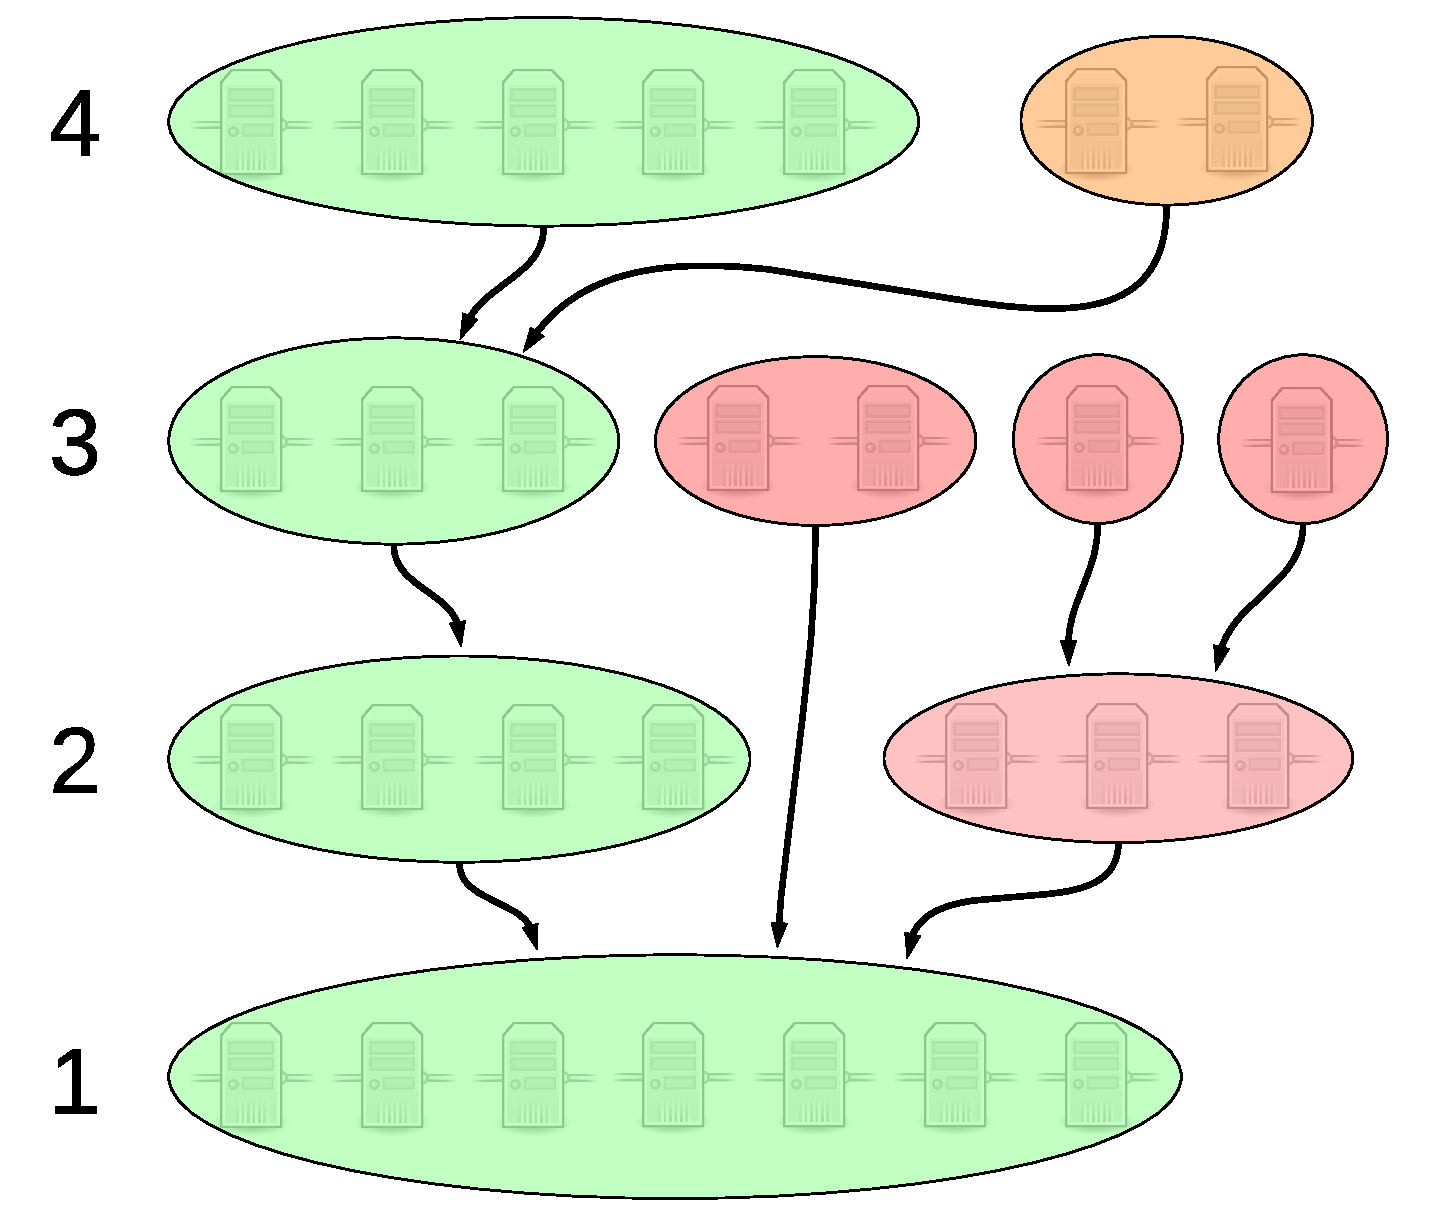
\includegraphics[width=0.7\linewidth]{../assets/images/LucidCharts/Page-chain2.pdf}
%	\caption{Each successive Quorum inherits the database from members of the previous Quorum. If the largest agreeing subset are at least semi-honest (green), then the master database will resist corruption from dishonest and colluding nodes (red) and malfunctioning nodes (orange).}
%	\label{fig:databaseInheritance}
%\end{figure}

Database updates are usually done in near real-time in a peer-to-peer fashion. At startup, OnioNS mirrors subscribe to new information by opening authenticated circuits to the Quorum and attempting to read from the circuit. All Quorum nodes subscribe to each other, forming a complete graph. Assuming that all mirrors are online and at least semi-honest, all mirrors will be processing the same ephemeral and main databases. However, some mirrors may drop offline temporarily or new ones may appear on the network, and these must synchronize with the network to update their databases. Mirrors select certain Quorum nodes to synchronize against by the following algorithm. Let Charlie be a mirror.

% todo: enough detail here?
\begin{enumerate}
	\item Charlie asks each Quorum node for $ \mathcal{H}(\mathit{database}_{ephemeral}) $ and $ \mathcal{H}(\mathit{database}_{main}) $.
	\item Charlie finds the largest group of Quorum nodes that return the same hashes.
	\item Charlie downloads the ephemeral and main databases from any of these nodes.
	\item Charlie verifies that $ \mathcal{H}(\mathit{database}_{ephemeral}) $ and $ \mathcal{H}(\mathit{database}_{main}) $ match the group's hashes.
	\item Charlie verifies the integrity of all records in both databases.
	\item Charlie merges the downloaded databases into his local databases.
\end{enumerate}

Quorum nodes that were temporarily offline conduct the same algorithm, but may also ask other Quorum nodes to replay new tickets so that they may update that database too. Non-Quorum mirrors subscribe to Quorum nodes according to the same algorithm.

% When hidden services transmit information to the Quorum, each Quorum node replays it to all subscribers. This allows all Quorum members to receive the same information even if the hidden service transmits to only some Quorum nodes.

\subsubsection{Ticket Generation} % done
\label{sec:ticketGeneration}

A hidden service operator, Bob, may enter into the OnioNS lottery by generating a ticket, containing a second-level domain name for his hidden service. The Quorum verifies the validity of his ticket and it may be further checked by mirrors and clients if his ticket wins the lottery, so Bob must follow this protocol to ensure that his ticket is accepted by all parties.

\begin{enumerate}
	\item Bob sets \emph{type} to ``ticket''.
	\item Bob provides the \emph{name} and \emph{subdomains} fields by specifying a second-level domain name and subdomain-destination pairs for his hidden service, respectively.
	\item Bob optionally sets \emph{contact} to his PGP key fingerprint.
	\item Bob sets \emph{rand} to $ \mathcal{G}(i) $.
	\item Bob fills \emph{nonce} with zeros.
	\item Bob sets \emph{pow} as $ \mathrm{PoW}(\mathit{c}) $, where $ \mathit{c} $ is $ \mathit{type} \concat \mathit{name} \concat \mathit{subdomains} \concat \mathit{contact} \concat \mathit{rand} \concat \mathit{nonce} $.
	\item Bob sets \emph{signature} as the output of $ S_{\mathit{RSA}}(m, r) $ where $ m = \mathit{c} \concat \mathit{pow} $ and $ r $ is Bob's private RSA key.
	\item Bob saves the PKCS.1 DER encoding of his RSA public key in \emph{pubHSKey}.
\end{enumerate}

Bob's ticket is valid when $ \mathit{pow}(\mathit{c} \concat \mathit{pow} \concat \mathit{signature}) \leq d $ where \emph{d} is a constant that specifies the work difficulty. We define this algorithm with the expectation that Bob must increment \emph{nonce}, re-perform $ \mathrm{PoW}(\mathit{c}) $ twice, and resign his ticket until the aforementioned formula is satisfied. Once this is the case, Bob sends his ticket to all Quorum nodes.

\subsubsection{Ticket Processing} % done

A Quorum node $ Q_{i,k} $ listens for tickets from hidden service operators. When a ticket $ t $ is received, $ Q_{i,k} $

\begin{enumerate}
	\item Rejects $ t $ if $ t $ is not valid according to the protocol described in section \ref{sec:ticketGeneration}.
	\item Rejects $ t $ if $ t $'s \emph{name} already exists in its lottery, ephemeral, or main databases.
	\item Rejects $ t $ if the hidden service does not have a descriptor in Tor's distributed hash table.
	\item Rejects $ t $ if the hidden service cannot answer an HTTP GET request.
	\item Rejects $ t $ if the response from an HTTP GET matches any other response from previous tickets.
	\item Otherwise, it accepts $ t $, records $ t $ in its lottery database, and sends $ t $ to all other Quorum nodes.
\end{enumerate}

\subsubsection{Lottery Management} % done

In section \ref{sec:ticketGeneration} we describe a proof-of-work (PoW) protocol that acts as a barrier-of-entry. It is straightforward to design a system where a name is awarded after the completion of this PoW; however such a system is vulnerable to attacks by adversaries with strong computational capabilities who may quickly register many names, as we described in section \ref{sec:adversaryPowers}. In an attempt to resolve this problem, we introduce a lottery-like system, managed by Quorum nodes.

The lottery starts at the formation of the Quorum. During the lottery, the Quorum accepts requests (or ``tickets'') for names for hidden services, creating a list $ T_{i} $. The lottery ends when $ Q_{i} $ is cycled to $ Q_{i + 1} $. At this time, each node in $ Q_{i} $ performs the following algorithm. Let Charlie $ \in Q_{i} $.

\begin{enumerate} % todo: use define character instead of =
	\item Charlie publishes $ T_{i} $ to all subscribers.
	\item For each $ T_{i}(k) \in T_{i} $, Charlie computes $ V_{i}(k) = \mathrm{count}(T_{i}(k) \oplus G_{i + 1})$, where $ \mathrm{count}(x) $ counts the number of $ 1 $ bits in $ x $.
	\item Charlie sorts $ V_{i} $ in descending order.
	\item Charlie sets the list of winners, $ W_{i} $, to the hidden services corresponding to the first $ M $ members of $ V_{i} $, where $ M $ is a fixed number that we define in section \ref{sec:lotteryWinners}.
	\item Charlie merges $ W_{i} $ into his main database, letting them receive names.
\end{enumerate}

All mirrors or other parties may verify $ W_{i} $ and update their main database accordingly through the same protocol because $ T_{i} $ is now public. As this algorithm occurs at 00:00 UTC, mirrors then update their Merkle root hash per the protocol described in section \ref{sec:qQualification}.

In order to defend against the one-to-many and many-to-one attacks described in section \ref{sec:useCases}, each Quorum node only accepts the first ticket per hidden service and the first ticket per name. A many-to-many (either ``land rush'' or denial-of-registration) attack primarily increases the chances of the adversary winning names. However, our countermeasure is straightforward. First, the Quorum remembers a value $ \max(\mathrm{size}(T)) $, representing the highest number of tickets received by any past Quorum. Then, if $ Q_{i} $ receives more tickets than this amount, $ Q_{i} $ tells $ Q_{i + 1} $ to increase the difficulty of ticket generation according to the formula $ \frac{\max(\mathrm{size}(T))}{\mathrm{size}(T_{i})} $. The increase in ticket difficulty reduces the impact of the attack in the next lottery under our assumptions, as we detail in section \ref{sec:lotteryWinners}.

%Quorum ends when G(t+1) is actually published. 
%
%All reveals available so G(t) can be calculated
%G(t) first revealed
%
%or Quorum rotation - 1 day, then G(t) first revealed?

% accept only first for pubKey and first for name

% However, an attacker who is not a dirauth should not be able to influence the outcome at all.

% The reveal phase lasts 12 hours, and most authorities will send their reveal value on the first round of the reveal phase. This means that an attacker can predict the final shared random value about 12 hours before it's generated.

%\begin{figure}[h]
%	\centering
%	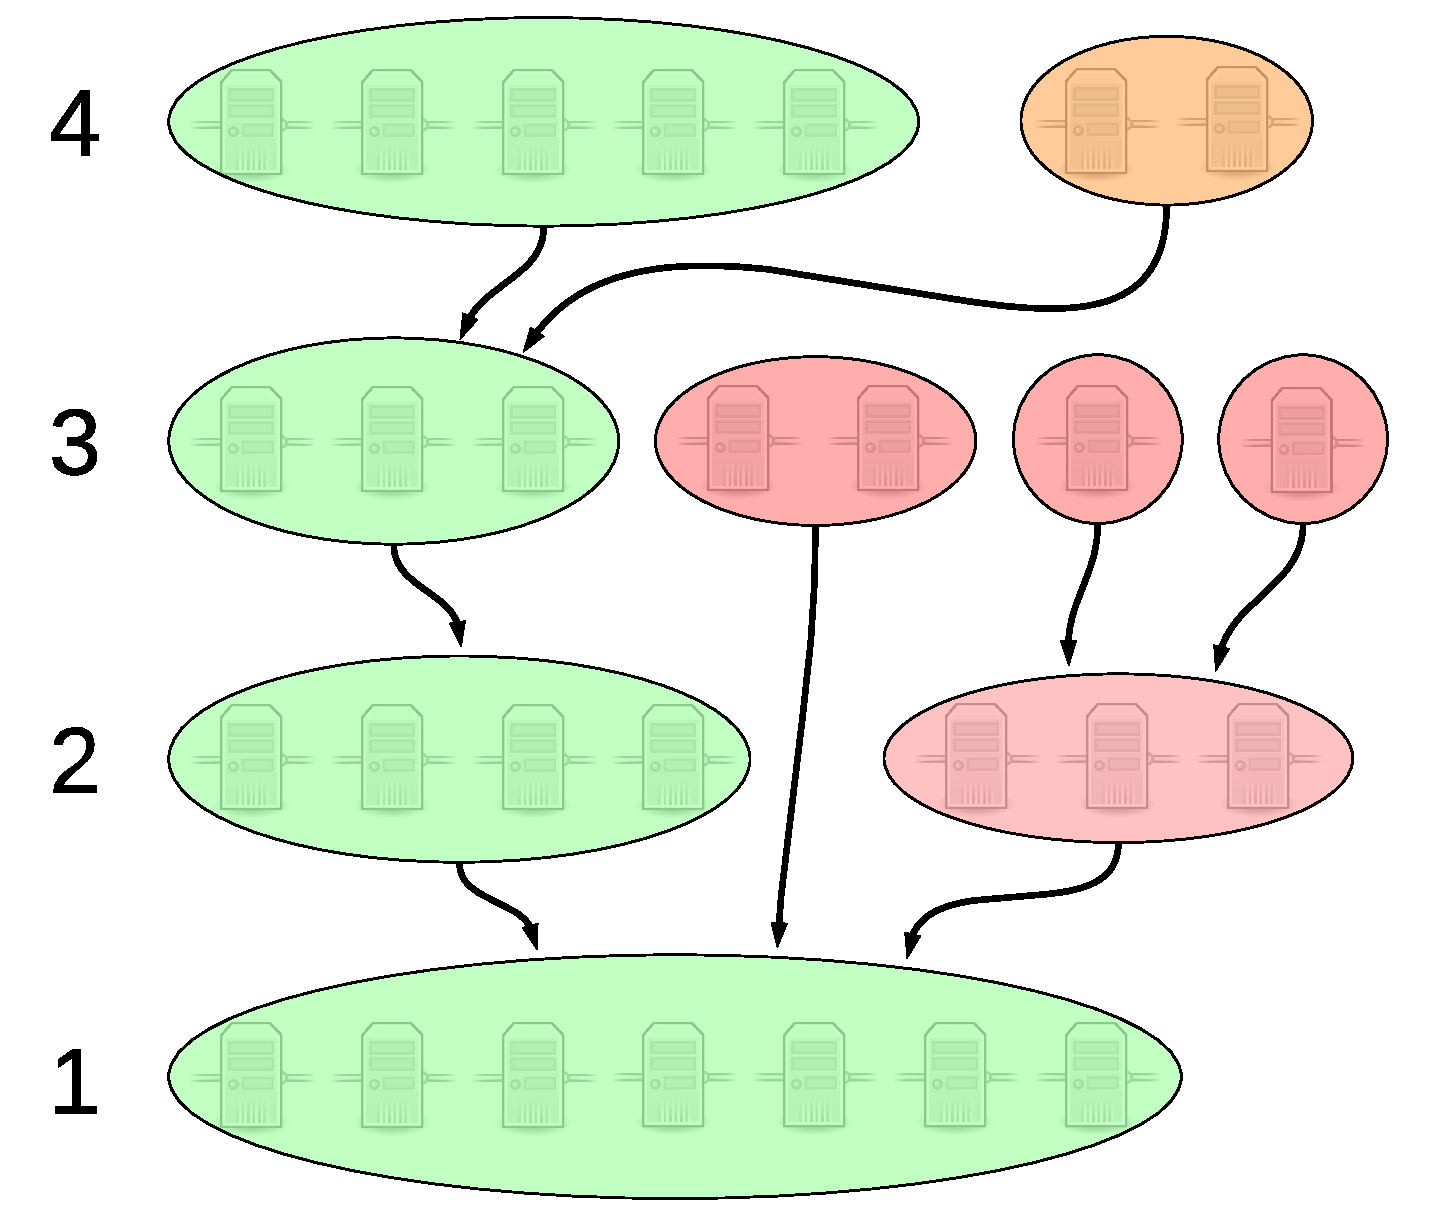
\includegraphics[width=0.4\linewidth]{../assets/images/LucidCharts/Page-chain2.pdf}
%	\caption{THIS IS A PLACEHOLDER IMAGE. TODO: create diagram of lottery-results timeline. The responsibilities of each Quorum are divided into two distinct parts: first, a lottery period where ``tickets'' are accepted and recorded; and second, a naming period where a fixed number of applicants receive names. The beginning of the Quorum and the lottery coincides with the publication of $ \mathcal{G}(t) $ in the consensus (section \ref{sec:rngProcess}) while the beginning of the naming period corresponds to the appearance of $ \mathcal{G}(t) $ by the directory authorities.}
%	\label{fig:lotteryTimeline}
%\end{figure}

\subsubsection{Record Operations} % done
\label{sec:recordOps}

% todo: I'd like to remove PoW from records, but then how would clients verify that the work was done? Would they get the original ticket too?
% at the current or original PoW difficulty? How is this handled? -maybe unnecessary detail

OnioNS also supports common operations on names. Owners of named hidden services may construct modify, renew, transfer, or delete records and issue the records to the Quorum. Once received, mirrors add these records to their ephemeral database. These records can be send to and authenticated by clients within 24 hours, as mirrors merge their ephemeral database into their main database and update their Merkle root publication at 00:00 UTC every day. In all cases, Bob sets the \emph{type} field to the appropriate record type.

Bob can modify his registration by changing either his \emph{subdomains} or \emph{contact} fields. Bob may also transfer the registration to a new owner by issuing a transfer record, which contains \emph{recipientKey}, the public RSA key of the new hidden service. Bob may also relinquish control of his name by issuing a delete record. Bob does not need to recompute proof-of-work for any of these records, so all parties ignore the \emph{pow} field, and these operations are cheap for the Quorum to apply. However, OnioNS names expire after 30 days, so name owners must periodically renew registrations to maintain ownership. This can be done by issuing a renew ticket with an $ \mathcal{G}(i) $.

%todo: analysis: non-winners will likely try again. Won't this impact the PoW-difficulty adjustment?
	
\subsubsection{Authenticated Denial-of-Existence} % todo
\label{sec:authDenial}

We described in section \ref{sec:authDenialIntro} that a malicious name server may forge a response or may falsely claim non-existence of a name. These are attack vectors that remain open by naming systems that do not provide authentication mechanisms. We use a Merkle tree \cite{merkle1988digital} to defend against these attacks with minimal networking costs. All mirrors, including Quorum nodes, perform this algorithm.

\begin{enumerate}
	\item Charlie fills an array list $ l $ with the $ r_{i}(\mathit{name}) \concat \mathcal{H}(r_{i}) $ for each Record $ r_{i} $ received from hidden services.
	\item Charlie sorts \emph{arr} by the $ \mathit{name} $ field.
	\item Charlie constructs a Merkle tree $ T $ from $ l $.
	\item Charlie publishes the root hash of $ T $ in the consensus as described in section \ref{sec:qQualification}.
\end{enumerate}

We note that a sorted Merkle tree does not support dynamic record updates and must be rebuilt at each update. While similar data structures exist that support proof of existence and non-existence and allow efficient updates, such as a skip list \cite{goodrich2001implementation}, these structures are significantly more complicated. We consider it sufficient to use a Merkle tree as it is only rebuilt once per day in $ \mathcal{O}(n \dot \mathrm{log}(n)) $ time.

%As the \mathit{name} field of each Record is globally unique, we may reference each Record by its \mathit{name}, which saves space. The Merkle tree also 

% As Records contain both second-level domains and their subdomains, $ T $ needs only contain $ c $ to reference all domains in $ r $, which further saves space. Then during a Domain Query Alice may use $ T $ to authenticate a domain $ d $ and verify non-existence for a Record $ r $. The Merkle tree also prevents phishing attacks from Charlie; the tree allows Alice to verify the mappings in $ r $ and the uniqueness of $ d $. The signatures from the Quorum allow her to verify the tree's authenticity. Quorum nodes maintaining identical Pages will sign the same Merkle tree root, so Alice needs to obtain only one subtree and the root signatures by every Quorum node from Charlie.

%Quorum nodes must also periodically regenerate and resign the Merkle tree described in \ref{sec:authDenial} and send the signature to all Quorum nodes and to all subscribers.

% The Quorum must regenerate $ T $ every $ \Delta T $ hours to include new Records. Then Alice needs only fetch the signatures on $ T $ at least every $ \Delta T $ hours to ensure that she can authenticate new Records during the Domain Query. Thus $ \Delta T $ is the primary factor in the speed of Record propagation: Alice cannot authenticate or verify denial-of-existence claims on Records newer than $ \Delta T $. Alice must also fetch the $ L_{Q} $ signature from all Quorum nodes and assert that $ T $ is signed by the largest set of nodes maintaining the same Page, in correspondence with our security assumptions.

% 

\subsubsection{Domain Query} % done

Alice only needs Bob's ticket or his latest record to contact Bob by his meaningful name. She then uses the Merkle tree structure to verify that her name server responds with the correct ticket or record, or to achieve authenticated denial-of-existence if her query has no corresponding data structure. Let Alice type a domain $ d $ into the Tor Browser.

\begin{enumerate}
	\item Alice contacts a name server Charlie via his hidden service.
	\item \label{step:ask} Alice asks Charlie for a ticket or record $ r $ containing $ d $.
	\item Charlie extracts the second-level name $ n $ from $ d $.
	\item If $ r $ exists, Charlie returns $ r $, the leaf node containing $ n $, and all the nodes from the leaf to the root and their sibling nodes.
	\item If $ r $ does not exist, Charlie returns two adjacent leaves $ a $ and $ b $ (and the nodes on their paths and siblings) such that $ a(\mathit{name}) < n < b(\mathit{name}) $, or in the boundary cases that $ a $ is undefined and $ b $ is the left-most leaf or $ b $ is undefined and $ a $ is the right-most leaf.
	\item Alice verifies the authenticity or non-existence of $ r $ by 
		\begin{enumerate}
			\item Asserting that $ n $ is either contained in the subtree or that $ n $ is spanned by the subtree leaves, respectively.
			\item Asserting the correctness of the hashes in the subtree.
			\item Asserting that the root hash matches the hash published by the largest agreeing set of Quorum nodes. %todo: does this last bit match database inheritance?
		\end{enumerate}
	\item If these assertions fail, Alice knows that Charlie is dishonest and she must repeat this protocol with a different mirror.
	\item If $ d $ in $ r $ points to a domain $ d_{2} $ which has a .tor pseudo-TLD, Alice jumps to \ref{step:ask} and queries for $ d_{2} $.
	\item Alice computes Bob's .onion address from $ r(\mathit{pubHSKey}) $ and contacts him in the hidden service protocol.
\end{enumerate}

While Alice can verify the authenticity and uniqueness of $ r $ by synchronize against the OnioNS network and downloading the database from the Quorum, but this is impractical in most environments. Tor's median circuit speed is often less than 4 Mbit/s, \cite{TorMetrics} so for the sake of convenience data transfer must be minimized. Therefore Alice can simply fetch minimal information and rely on her existing trust of members of the Tor network.

\subsubsection{Onion Query} % done

OnioNS also supports reverse-hostname lookups. In an Onion Query, Alice issues a hidden service address \emph{addr} to Charlie and receives back all Records that have \emph{addr} as either the owner or as a destination in their \emph{subdomain}. Alice may obtain additional verification on the results by issuing Domain Queries on the source .tor domains. We do not anticipate Onion Queries to have significant practical value, but they complete the symmetry of lookups and allow OnioNS domain names to have Forward-Confirmed Reverse DNS matches. We suggest caching destination hidden service addresses in a digital tree (trie) to accelerate this lookup; a trie turns the lookup from $ \mathcal{O}(n) $ to $ \mathcal{O}(1) $, while requiring $ \mathcal{O}(n) $ time and $ \mathcal{O}(n) $ space to pre-compute the cache.




%In simple terms, the essential idea is that many HSs can buy a lottery ticket for permission to claim a name, but later only a fix number of them actually get this permission. I assume that each HS will only make one lottery ticket for itself, though I realize that in this type of lottery, it's advantageous to buy many tickets in an attempt the chances of winning. In my scheme this results in a more expensive lottery ticket, which primarily affects the person who bought many tickets, thus the system self-adjusts to defend against a resource-rich adversary.

%In some more detail, let each HS create a ticket for permission to claim a name for itself. The ticket requires PoW to create but does not contain the desired name. The Quorum collects all the tickets and after some time compares the tickets to the latest shared randomness value. The closest Y applications are then allowed to claim a name, which they can then do. The key to the scheme is that nobody can know the shared randomness value in advance and that makes it a sort of lottery where Y winners are found once the random value is revealed. The system remembers the highest number of tickets received; if this number is exceeded the difficulty of the PoW increases proportionally, but the difficulty is never decreased. A well-resourced adversary might create many tickets in order to increase their chances, and while this might work once, in the next round it's harder to repeat the attack. This scheme also means that the system adjusts in response to an increase in average computational speed over time (often confused with Moore's Law).

%To clarify, a ticket can be compared to the shared random value by counting the number of "1" bits in A & V, where A is a ticket and "&" is the bitwise AND operation. Quorum nodes then sort the tickets by this comparison and allow the top Y HSs to claim a name. I chose this over a simpler comparison scheme, such as the absolute value of A - V, because this latter formula is easily exploitable.

% The idea here is that although everyone gets a proportionally-higher increase in PoW difficulty, it's acceptable by innocent parties (an extra 36 minutes is not that much) but the attacker now has to spend 48 hour of CPU (18 more hours) to get 30 tickets. If the attacker has a fixed budget for 30 hours of CPU time he'll be unable to make 30 tickets in lottery 3, but rather only 30/1.6=18. The difficulty never decreases, so if the number of tickets in the lottery is blinded from everyone except the Quorum, a point will be reached where the statistics are no longer in the attacker's favor, leading him to conclude that it's no longer worth it.

% Finally, an attacker might want to create many tickets in order to register many names or to increase the chances of registering a single name. Although it's very hard to stop the former attack, my lottery system rate-limits registrations and makes the attack expensive and minimizes the damage. The latter attack can be prevented by having each ticket contain a blinded name (by hashing the name) which winners must reveal in order to claim the name. Because a hash is used, the reveal can be applied to all tickets and any duplicates can be discarded, then the lottery can be repeated until a unique set of winners is chosen. 


%While the anonymous nature of hidden services makes it extremely difficult to distinguish 

%It is not easy to design a system that is resistant to this 
%
%
%land rushes and en-masse domain squatting by  (section \ref{sec:adversaryPowers}). 
%
%
%We listed this attack in section \ref{sec:adversaryPowers} and as a counter-measure we introduce a lottery-like system. While a h
%
%While it is straightforward to design a system 
%
%The protocol described in In section \ref{sec:RecordGeneration} we describe a hidden service operator can claim a name for his hidden 
%

%
%A \textbf{Page} contains $ \mathit{prevHash} $, set to $ \mathcal{H}(\mathit{prevHash} \concat \mathit{recordList} \concat \mathit{rand}) $ of some previous Page; $ \mathit{recordList} $, a \\ deterministically-sorted array list of Records; $ \mathit{rand} $, the output of $ \mathcal{G}(t) $ at the current time; $ \mathit{fingerprint} $, the Tor fingerprint of the router maintaining this Page; and $ \mathit{pageSig} $, the output of  $ S_{\mathit{ed}}(\mathcal{H}(\mathit{prevHash} \concat \mathit{recordList} \concat \mathit{rand}), e) $ where $ e $ is the router's private Ed25519 key.
%
%$ \mathit{prevHash} $ links Pages over time, forming an append-only public ledger known as a Pagechain. In contrast to existing cryptocurrencies such as Namecoin, we bound the Pagechain to a finite length, forcing hidden service operators to renew their domain periodically to avoid it being dropped from the network. In correspondence with our security assumptions, $ \mathit{prevHash} $ must reference a Page that is both valid and maintained by the largest number of Quorum members whom we assume are at least semi-honest, as illustrated in Figure \ref{fig:sideChains}. As $ \mathit{prevHash} $ does not include the router-specific $ \mathit{fingerprint} $ and $ \mathit{pageSig} $ fields, $ \mathit{prevHash} $ is equal across all Quorum members maintaining that Page.

%\setlength{\belowcaptionskip}{-10pt}

% infrastructure (Authorative servers) (server management), registration process

%\subsection{Overview}
%
%We propose the Onion Name System (OnioNS) as an abstraction layer to hidden service addresses and introduce ``.tor'' as a new pseudo-TLD for this purpose.
%
%forget signing the same page/database, signing the same Merkle root?
%	include last Record's name + root sig in consensus
%prop224
%
%% \cite{jacobs2014providing} was
%
%%$ P (Q_{i}) = \frac{Q_{i}(w)}{\sum_{j=0}^{\concat R \concat} R_{j}(w)} $
%
% First, Bob generates and self-signs a \emph{Record}, containing a meaningful second-level domain name and his public key $ \mathcal{P}_{B} $. Without loss of generality, let this be ``example.tor $ \rightarrow $ onions55e7yam27n.onion''. We introduce a proof-of-work scheme that requires Bob to expend computational and memory resources to claim ``example.tor''; the protocol allows Bob to claim a meaningful name in a distributed environment while remaining anonymous. Proof-of-work systems are noteworthy for their asymmetry: they require the issuer to spend effort to find an answer to a moderately hard computational problem, but once solved can be easily verified correct by any recipient. The requirement of proof-of-work fulfils three main purposes:
%
%\begin{enumerate}
%	\item Significantly reduces the threat of DoS flood attack.
%	\item Introduces a barrier-of-entry that encourages the utilization of domain names and the availability of the underlying hidden services.
%	\item Increases the difficulty of domain squatting.
%\end{enumerate}
%
%Second, Bob uses a Tor circuit to anonymously transmit his Record to an authoritative short-lived random subset of OnioNS servers, known as the Quorum, inside the Tor network. The Quorum archive Bob's Record in a sequential public ledger known as a Pagechain, of which each OnioNS node holds their own local copy. Bob's Record is received by all Quorum nodes and share signatures of their knowledge with each other, so they maintain a common database. Quorum nodes are not name servers, so let Charlie be a name server outside the Quorum and assume that Charlie stays synchronized with the Quorum.
%
%Third, Alice, uses a Tor circuit to anonymously ask Charlie for ``example.tor''. Alice receives Bob's Record, verifies its signature and proof-of-work, and uses $ \mathcal{P}_{B} $ to contact Bob via Tor's hidden service protocol. As Bob's Record is self-signed and contains $ \mathcal{P}_{B} $, Alice can verify the Record's authenticity relative to $ \mathcal{P}_{B} $. In this way, Alice does not have to resort to using ``onions55e7yam27n.onion'', rather that Bob can be successfully referenced by ``example.tor''. We illustrate the OnioNS overview in Figure \ref{fig:basicDesign}.



%mention that consensus weight is tied to path selection




\section{Security Analysis}
\label{sec:Analysis}

In this section, we analyse the security of the OnioNS system with regard to our security goals. First, the registrations and client queries are anonymous because they occur over a Tor circuit, which we assume provides privacy and anonymity. No identifiable information is leaked from the data contents as well. Second, registrations are authenticable, which can be reduced to the security of the Merkle hash tree and to the assumption that the largest subset of Quorum nodes are honest. We verify this assumption in section \ref{sec:QSelection} and \ref{sec:qSize}. Domain uniqueness also stems from the above assumption, relying on honesty of Quorum nodes to avoid collisions. Quorum selection is a random process assuming security of the commitment algorithm run by the directory authorities, which we analyse in section \ref{sec:RandGeneration}. We also highlight the potential for the leakage of the .tor pseudo-TLD on the Internet DNS.

\subsection{Quorum Selection}
\label{sec:QSelection}

In section \ref{sec:threatModel}, we assume that an attacker, Eve, controls some fixed $ f_{E} $ fraction of routers on the Tor network. Quorum selection may be considered as an $ L_{Q} $-sized random sample taken from an $ L_{T} $-sized population without replacement, where the population contains $ L_{T} \cdot f_{E} $ entities that we assume are compromised and colluding. If our selection includes $ L_{E} $ Eve-controlled routers, then Eve controls the Quorum if either $ > \frac{L_{Q} - L_{E}}{2} $ honest Quorum nodes disagree or if $ L_{E} > \frac{L_{Q}}{2} $. The former scenario is hard to model theoretically or in simulation, but the probability of the latter can be statistically calculated. The Quorum is rotated every $ \Delta q $ days, so we must consider the implications of selections for both $ L_{Q} $ and $ \Delta q $.

\subsubsection{Quorum Size}
\label{sec:qSize}

The probability that Eve controls $ L_{E} $ Quorum nodes is given by the hypergeometric distribution, whose probability mass function is shown in Equation \ref{eq:hypergeoPMF}.

\begin{align}
	\mathrm{Pr}(L_{E}) &= \frac{\binom{L_{T} \cdot f_{E}}{L_{E}}\binom{L_{T} - L_{T} \cdot f_{E}}{L_{Q} - L_{E}}}{\binom{L_{T}}{L_{Q}}}
	\label{eq:hypergeoPMF}
	\\
	\mathrm{Pr}(L_{E} > \frac{L_{Q}}{2}) &= \displaystyle\sum_{i=\ceil{\frac{L_{Q}}{2}}}^{L_{Q}} \frac{\binom{L_{T} \cdot f_{E}}{i}\binom{L_{T} - L_{T} \cdot f_{E}}{L_{Q} - i}}{\binom{L_{T}}{L_{Q}}}
	\label{eq:compromiseProb}
\end{align}

If all Quorum Candidates have an equal probability of selection, then the probability that $ L_{E} > \frac{L_{Q}}{2} $ is given by the $p$-value of the hypergeometric test for over-representation, expressed in Equation \ref{eq:compromiseProb}. Odd choices for $ L_{Q} $ prevents the network from splintering in the event that the Quorum is evenly split across two Pages. We provide the statistical calculations of Equation \ref{eq:compromiseProb} for various Quorum sizes in Figure \ref{fig:quorumUnweightedMajority}.

\begin{figure}[h]
	\centering
	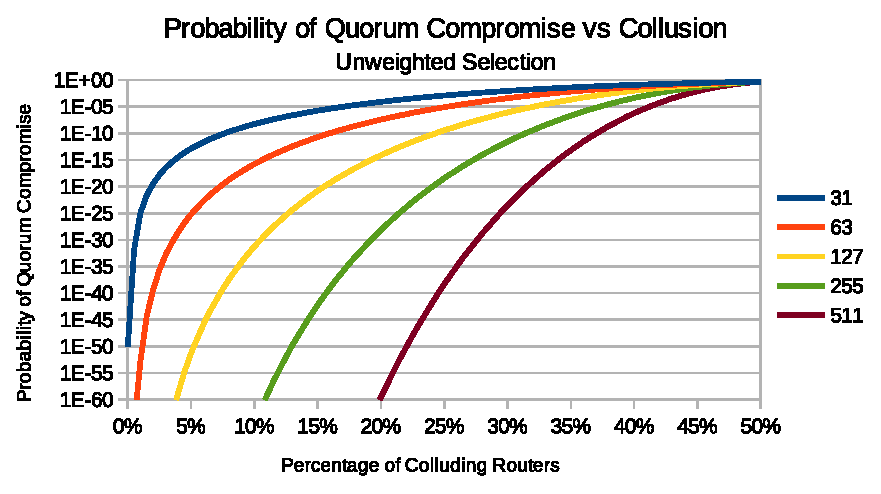
\includegraphics[width=\linewidth]{../assets/analysis/QuorumSelectionUnweighted.eps}
	\caption{The values for $ \mathrm{Pr}(L_{E} > \frac{L_{Q}}{2}) $ for Quorum sizes of 31, 63, 127, 255, and 511. All probabilities exceed 0.5 when more than 50 percent of the Tor network is under Eve's control. We set our population to 4540 routers; the average number of routers with the Fast, Stable, and Running flags across all consensuses in July 2015 \cite{TorMetrics}.}
	\label{fig:quorumUnweightedMajority}
\end{figure}

In practice Tor routers do not have equal consensus weight, thus Quorum selection from the pool of Quorum Candidates is heavily skewed by the distribution of consensus weight. The selection probabilities of routers with the Fast, Stable, and Running flags closely follows an exponentially-decreasing distribution, as shown in Figure \ref{fig:weightDist}. The figure suggests that the Tor network contains a low number of high-end routers and a large number of low-end routers.

\begin{figure}[h]
	\centering
	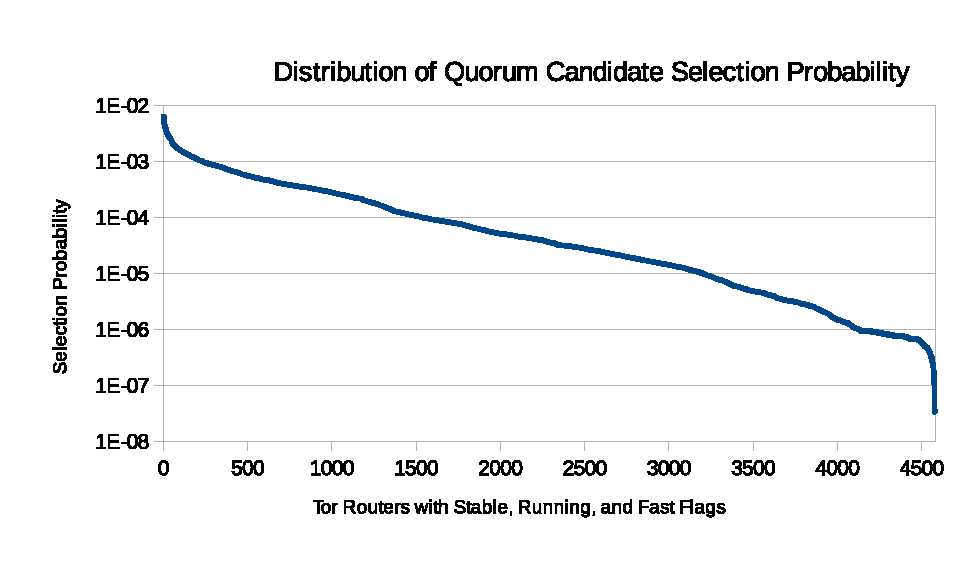
\includegraphics[width=\linewidth]{../assets/analysis/QuorumCandidateWeights.eps}
	\caption{The selection probabilities of Quorum Candidates averaged across all consensuses in July 2015. These probabilities closely follow an exponential distribution; a exponential trendline models it with $ R^{2} = 0.9884 $.}
	\label{fig:weightDist}
\end{figure}

We now re-examine Equation \ref{eq:compromiseProb} with regard to this distribution of consensus weight. Consider that the hypergeometric distribution describes the probability of selecting $ k $ Eve-controlled routers in an $ L_{Q} $-sized Quorum from an $ N $-sized population containing $ K $ Eve-controlled routers. Let $ L(x) $ be the probability distribution of selecting a router whose consensus weight is at the lowest $ x $ percentile. Then the probability of compromise is given by Equation \ref{eq:compromiseWeighted} where $ K $, the expected number of routers in a population of size $ N $, is given by Equation \ref{eq:compromiseK}, and $ R $ is the probability that routers outside $ L(x) $ are compromised. Since $ L(x) $ describes probabilities and $ N $ must be a natural number, ($ N \in \mathbb{N} $) this approach provides an approximation of the probability of compromise.

We illustrate the probabilities against discrete values of $ x $ and various Quorum sizes in Figure \ref{fig:quorumWeightedMajority} using $ N = 4540 $, consistent with the population in Figure \ref{fig:quorumUnweightedMajority}.

\begin{align}
	K &= N \cdot \left( \int_0^x(L(x)) + R \cdot \int_x^1(L(x)) \right)
	\label{eq:compromiseK}
	\\
	\mathrm{Pr}(L_{E} > \frac{L_{Q}}{2}) &= \displaystyle\sum_{i=\ceil{\frac{L_{Q}}{2}}}^{L_{Q}} \frac{\binom{K}{i}\binom{N - K}{L_{Q} - i}}{\binom{N}{L_{Q}}}
	\label{eq:compromiseWeighted}
\end{align}

\begin{figure}[h]
	\centering
	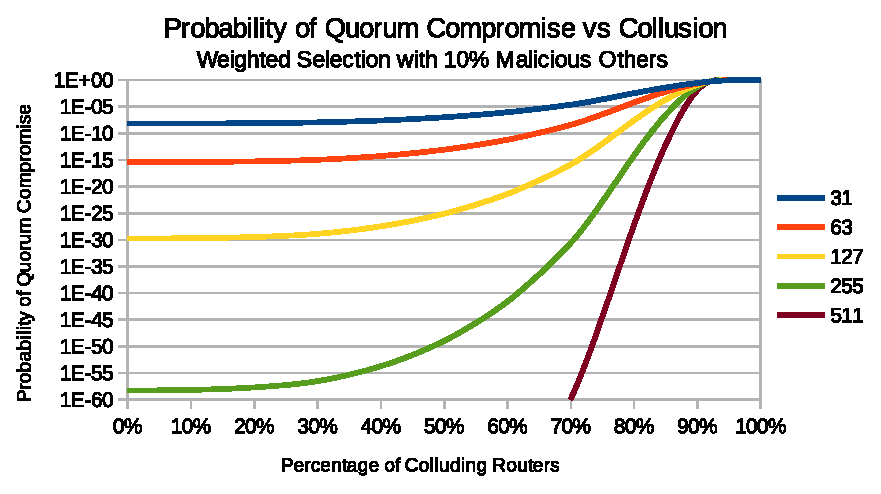
\includegraphics[width=\linewidth]{../assets/analysis/QuorumSelectionWeighted10.eps}
	\caption{The values for $ \mathrm{Pr}(L_{E} > \frac{L_{Q}}{2}) $ from Equation \ref{eq:compromiseWeighted} for various Quorum sizes. We assume that all routers $ \in L(x) $ are under Eve's control, while routers $ \notin L(x) $ have a 10 percent chance of being under Eve's control.}
	\label{fig:quorumWeightedMajority}
\end{figure}

In contrast to Figure \ref{fig:quorumUnweightedMajority} which demonstrates that an unweighted selection leads to a high probability of compromise with small levels of collusion, Figure \ref{fig:quorumWeightedMajority} suggests that biasing Quorum selection by consensus weight provides a strong defence against large-scale Sybil attacks. Indeed, even when 60 percent of the low-end Quorum Candidates are malicious, most Quorum sizes produce negligible probabilities of compromise. We consider it reasonable to assume that low-end routers are under Eve's control; these routers are the cheapest and logistically easiest to operate. Our approach remains resistant to this attack: these routers will be included in the Quorum very infrequently because of their low consensus weight.

Small Quorums are also more susceptible to node downtime or distributed denial-of-service (DDoS) attacks. Figure \ref{fig:quorumWeightedMajority} shows that the choices of $ L_{Q} = 31 $ is suboptimal; it is more easily compromised even with low levels of collusion. $ L_{Q} = 63 $ is more resistant, but not significantly more so. We therefore recommend $ L_{Q} \geq 127 $.

\subsubsection{Quorum Rotation}
\label{sec:qRotation}

In section \ref{sec:threatModel}, we assume that $ f_{E} $ is fixed and does not increase in response to the inclusion of OnioNS on the Tor network. If we also assume that $ L_{T} $ is fixed, then we can examine the impact of choices for $ \Delta q $ and calculate the probability of Eve compromising \emph{any} Quorum over a period of time $ t $. Shorter-lived Quorums reduces the disruption timeline for a malicious Quorum and are less susceptible to the disruption caused by nodes experiencing downtime or disappearing entirely from the network. Eve's cumulative chances of compromising any Quorum is given by $ 1 - (1 - f_{c})^{\frac{t}{\Delta q}} $ where $ f_{c} $ is Eve's chances of compromising a single Quorum. We estimate this over 10 years in Figure \ref{fig:cumulativeProbability}.

\begin{figure}[h]
	\centering
	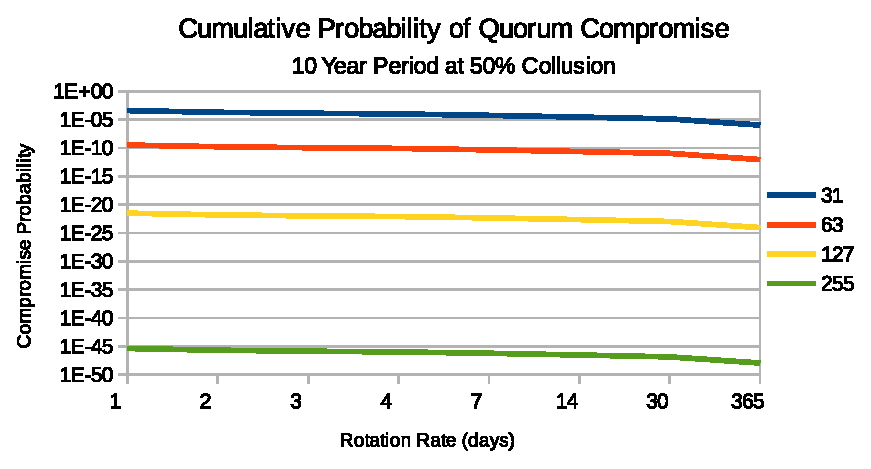
\includegraphics[width=\linewidth]{../assets/analysis/CumulativeMaliciousQuorumNew.eps}
	\caption{The cumulative probability that Eve controls any Quorum at different rotation rates over 10 years at $ f_{E} = 50 $ for Quorum sizes 31, 63, 127, and 255. We base these statistics on the probabilities from Figure \ref{fig:quorumWeightedMajority} at 50 percent collusion.}
	\label{fig:cumulativeProbability}
\end{figure}

%It also supports our earlier conclusion that the choices of $ L_{Q} = 31 $ and $ L_{Q} = 63 $ are suboptimal.
Figure \ref{fig:cumulativeProbability} suggests that although larger values of $ \Delta q $ positively impact security, the choice of $ L_{Q} $ is more significant. Furthermore, even "Stable" routers in the Tor network may be too unstable for very high values of $ \Delta q $. Therefore, based on Figure \ref{fig:cumulativeProbability}, we further reiterate our recommendation of $ L_{Q} \geq 127 $ and suggest $ \Delta q = 7 $. Although a malicious Quorum would have the capabilities to deploy a variety of attacks on the network, the proper selections of $ L_{Q} $ and $ \Delta q $ reduces the likelihood of this occurring to near-zero probabilities. We consider this a stronger solution than introducing countermeasures to specific Quorum-level attacks.

\subsubsection{Global Randomness}
\label{sec:RandGeneration}

We implement $ \mathcal{G}(t) $ using a commitment scheme run by Tor directory authorities \cite{GouletCommitReveal}. Commitment protocols have been studied in other works \cite{rivest1999unconditionally}\cite{naor1990bit}, have many interesting applications, and are well understood. If all parties are at least semi-honest then the commitment protocols generally display correctness, privacy, and binding. 

However, if some participants are malicious, they demonstrate known weaknesses. Namely, while reveals must demonstrably match commits, each participant may choose to reveal or not. If they do not reveal, their value is lost and the protocol produces a different output. If Eve controls $ b $ participants, she can make this choice with each participant in turn, allowing $ 2^{b} $ different outcomes. Goulet and Kadianakis' directory authority commitment scheme is particularly vulnerable to this attack because the reveals are public for approximately 12 hours before the final random value is published. However, as there are currently only nine directory authorities and the security of the Tor network rests on the assumption that five or more of them are at least semi-honest, the commitment scheme has at most $ 2^{4} = 16 $ different outcomes in the worst case without violation of our assumptions. 

Given the statistical calculations and the safety margin introduced by the recommendations in section \ref{sec:qSize}, we do not consider this a significant threat to our system and conclude that the Quorum Formation protocol is secure under our design assumptions. The unpredictability of the reveals and the low probability of compromise shown in Figures \ref{fig:quorumWeightedMajority} and \ref{fig:cumulativeProbability} provides the strongest defence against Quorum-level attacks.

 TO REWRITE: The security analysis in \cite{GouletCommitReveal} suggests that $ \mathcal{G}(i) $ is expected to be computable 12 hours prior to $ \mathcal{G}(i) $'s publication; thus to avoid consensus manipulation attacks, such as the adding or removing of colluding routers in order to manipulate this algorithm, we apply $ \mathcal{G}(i) $ from $ \mathit{cd}_{a} $ to the network status described in $ \mathit{cd}_{b} $.
\subsection{Number of Winners in Lottery}
\label{sec:lotteryWinners}

 As $ T_{i} $ is initially blinded, it is difficult for the adversary to determine in advance if this threshold is reached. This scheme also means that the system adapts in response to an increase in global average computational speed as the barrier-of-entry becomes too low.

\subsection{Outsourcing Record Generation}

In the Record Generation protocol, we intentionally included the scrypt calculation inside the signing step in order to require Bob to run scrypt himself, preventing him from utilizing large-scale compute engines such as the Amazon Cloud. However, our protocol does not entirely prevent Bob from outsourcing this expensive computation to a secondary resource, Craig, in all cases. We assume that Craig does not have Bob's private key. Then,

\begin{enumerate}
	\item Bob creates an initial Record $ R $ and completes the \emph{type}, \emph{name}, \emph{subdomains}, \emph{contact}, and \emph{rand} fields.
	\item Bob sends $ R $ to Craig.
	\item  Let $ \mathit{c} $ be $ \mathit{type} \concat \mathit{name} \concat \mathit{subdomains} \concat \mathit{contact} \concat \mathit{rand} $.
	\item Craig generates a random integer $ K $ and then for each iteration $ j $ from 0 to $ K $,
		\begin{enumerate}
			\item Craig increments \emph{nonce}.
			\item Craig sets \emph{PoW} as $ \mathrm{PoW}(\mathit{c} \concat \mathit{nonce}) $.
			\item Craig saves the new $ R $ as $ C_{j} $.
		\end{enumerate}
	\item Craig sends all $ C_{0 \le j \le K} $ to Bob.
	\item For each Record $ C_{0 \le j \le K} $ Bob computes
		\begin{enumerate}
			\item Bob sets \emph{pubHSKey} to his public RSA key.
			\item Bob sets \emph{signature} to $ S_{\mathit{RSA}}(m, r) $ where $ m = \mathit{c} \concat \mathit{nonce} \concat \mathit{pow} $ and $ r $ is Bob's private RSA key.
			\item Bob has found a valid Record if $ \mathcal{H}(\mathit{c} \concat \mathit{nonce} \concat \mathit{pow} \concat \mathit{signature}) \leq d $ where $ d $ is the difficult level.
		\end{enumerate}
\end{enumerate}

% todo: calculate chances of Craig computing a correct record

However, this ensures that Craig will with high probability compute more scrypt iterations than necessary; Craig cannot generate \emph{signature} and thus cannot compute if the hash is below the threshold. Moreover, the scrypt work incurs a cost onto Craig that must be compensated financially by Bob. Thus the Record Generation protocol always places a cost on Bob.

\subsection{DNS Leakage}

Accidental leakage of .tor lookups over the Internet DNS via human mistakes or misconfigured software may compromise user privacy. This vulnerability is not limited to OnioNS and applies to pseudo-TLD; Mohaisen and Thomas observed .onion lookups on root DNS servers at a frequency that corresponded to external global events and highlighting the human factor in those leakages \cite{thomasmeasuring}. Closing this leakage is difficult; arguably the simplest approach is to introduce whitelists or blacklists into common web browsers to prevent known pseudo-TLDs from being queried over the Internet DNS. Such changes are outside the scope of this work, but we highlight the potential for this attack.

\section{Evaluation}
\label{sec:Evaluation}

\subsection{Implementation}

We have build a reference implementation of the Onion Name System in C++11. We implemented the essential protocols for Bob, Charlie, and Alice. We divided our software into three parts: OnioNS-client, OnioNS-server, and OnioNS-HS, with OnioNS-common as a shared library dependency. We utilize several common libraries; Botan \cite{BotanLib} provides the implementation of our cryptographic operations, Boost Asio \cite{AsioLib} provides our networking engine, Stem provides abstraction for Tor control, and jsoncpp \cite{JsonCppLib} provides implementations of JSON encoding and decoding. We encode all the data structures in JSON; JSON is significantly more compact than XML, but retains user readability and its support of basic primitive types is highly applicable to our needs. 

OnioNS-HS is a small command-line utility that provides the capability for Bob to define a Record, make it valid, and then transmit it over a Tor circuit to a Quorum node. We provide flags to allow Bob to run the proof-of-work while inside a small VM or other restricted environment. OnioNS-HS then communicates with Tor's SOCKS port to send the Record to Quorum nodes.

OnioNS-server provides the main OnioNS functionality and is designed to run in the background with minimal configuration. We introduce a flag to specify whether the server is a Quorum node or a traditional Mirror. As a Mirror, it maintains a network connection and subscribes to OnioNS servers running as Quorum nodes. It utilizes OnioNS-common to distributes networking information and public keys by installing several JSON files.

The client-side software consists of three distinct pieces: onions-client, which connects to a Tor circuit over a Mirror and then listens on a TCP port on localhost for .tor domains; a Python script which waits for Tor stream requests, intercepts .tor domains, and sends them to the IPC port for resolution; and onions-tbb, which launches the Tor executable, onions-client, and then the Python script as child processes when the Tor Browser starts. The Python script reconfigures Tor to prevent it from auto-attaching network streams to circuits; instead, it filters stream requests and resolves .tor domains before letting Tor attach them, while instantly manually attaching streams for all other domains.

We created a Linux repository and used the Launchpad build system to package our software for several distributions. We designed the software with usability in mind: each aspect of the software runs with minimal configuration and management; the onions-client in particular integrates easily with the Tor Browser. Our code is available on Github under the Modified BSD License, matching Tor.

\subsection{Integration Test}

First, we started two OnioNS servers, a Quorum node and a Mirror. We created a hidden service for our project, \href{http://onions55e7yam27n.onion}{``onions55e7yam27n.onion''}, and generated a Record to claim ``example.tor''. Once the Record was complete, OnioNS-HS transmitted it over a Tor circuit to the Quorum node. The Mirror, as a subscriber to the Quorum node, also received, verified, and cached our Records.

Finally, we installed our client software into Tor Browser 5.5, a fork of Firefox 38.2.0 ESR. Once we launched the Tor Browser, the prepackaged Tor binary, onions-client, and the Python script started in the background. We entered ``example.tor'' into the Tor Browser, which caused Tor to fire a network stream event over its controller port. The Python script intercepted the .tor pseudo-TLD and sent the domain over IPC to onions-client. The client then issued a Domain Query to the Mirror for ``example.tor'' and resolved it to ``onions55e7yam27n.onion''. The Python script rewrote the stream request to ``onions55e7yam27n.onion'' before letting Tor attach it to a circuit. Tor then loaded our hidden service and returned our webpage back to the Tor Browser.

This process resulted in the Tor Browser transparently loading our hidden service under ``example.tor'' without requiring any further user interaction. We illustrate this result in Figure \ref{fig:prototypeExample}. The software performed asynchronously and allowed normal browsing to both the Internet and other hidden services, even while the OnioNS domain was resolving.

%\begin{figure}[h]
%	\centering
%	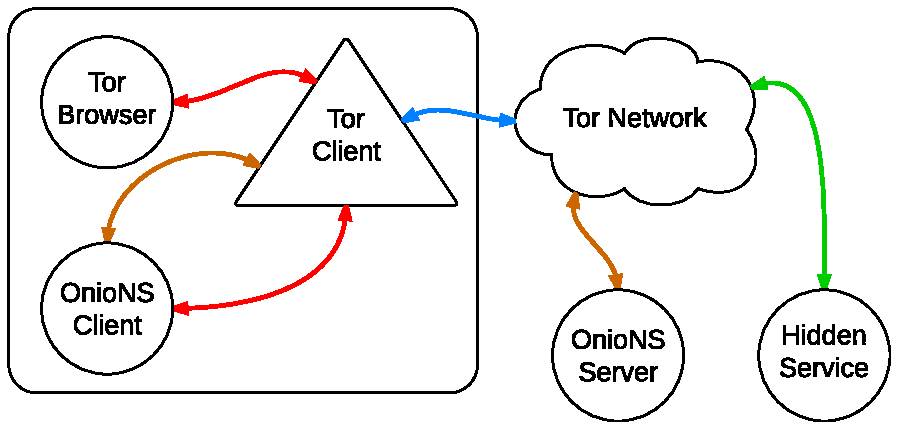
\includegraphics[width=0.6\linewidth]{../assets/images/LucidCharts/OnioNS_Prototype.pdf}
%	\caption{The unresolved .tor pseudo-TLD travels (red) from the Tor Browser to the OnioNS client. The client issues a Domain Query (orange) to a remote server, who returns a Record. The client returns the .onion address to Tor, which then contacts the HS (green).}
%	\label{fig:prototypeDiagram}
%\end{figure}

\begin{figure}[h]
	\centering
	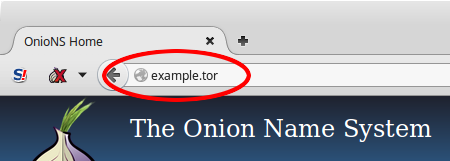
\includegraphics[width=\linewidth]{../assets/images/example.png}
	\caption{We load the OnioNS' hidden service, onions55e7yam27n.onion, transparently under the ``example.tor'' domain. The OnioNS software launches with the Tor Browser.}
	\label{fig:prototypeExample}
\end{figure}

\subsection{Results}

\subsubsection{Performance}

Our experiment involves two machines, A and B. Both were hosted on 1 Gbit connections on a university campus. Machine A has an Intel Core2 Quad Q9000 (Penryn architecture) @ 2.00 GHz CPU from late 2008 and Machine B has an Intel i7-2600K (Sandy Bridge architecture) @ 4.3 GHz CPU from 2011, representing low-end and medium-end consumer-grade computers, respectively.

We selected the parameters of scrypt such that it consumed 128 MB of RAM during operation. We consider this an affordable amount of RAM for low-end consumer-grade computers. We created a multi-threaded implementation of the Record Generation protocol and used all eight virtual CPU cores on Machine B to generate our Record. As expected, our RAM consumption scaled linearly with the number of scrypt instances executed in parallel; we observed approximately 1 GB of RAM consumption during Record Generation. We set our difficulty level so that Records took approximately six hours on average to become valid on Machine B.

We conducted several performance measurements for the Domain Queries.  We measured and averaged 200 samples of the CPU wall-time required for both machines to validate the Record.

\renewcommand{\arraystretch}{1.3}
\newcolumntype{L}[1]{>{\hsize=#1\hsize\raggedright\arraybackslash}X}%
\newcolumntype{R}[1]{>{\hsize=#1\hsize\raggedleft\arraybackslash}X}%
\newcolumntype{C}[2]{>{\hsize=#1\hsize\centering\arraybackslash}X}%
\begin{table}[h]
	\small
	\begin{tabularx}{\linewidth}{ | C{1} || C{1} || C{1} || }
		\hline
    \textbf{Description} & \textbf{A (ms)} & \textbf{B (ms)} \\ \hline
    Parsing JSON & 5.21 & 2.42 \\ \hline
	Validating scrypt & 448.184 & 294.963 \\ \hline
	$ V_{\mathit{RSA}}(m, E) $ & 6.35 & 2.74 \\ \hline
	Total Time & 459.744 & 300.123 \\ \hline
  	\end{tabularx}
\end{table}

As expected, Machine B outperformed Machine A in all instances and we observed that single iteration of scrypt dominated the total validation time. This is a CPU cost introduced to Tor clients, Mirrors, and Quorum nodes for each Record.

Clients must also check the Merkle root signatures from all $ L_{Q} $ Quorum nodes. We use Ed25519 to reduce the signature space requirements and CPU time required for verification: $ S_{\mathit{ed}}(m, e) $ signatures fit into 64 bytes and may be verified in batch form. Bernstein et al. reports that a quad-core Westmere-era CPU can generate 109,000 signatures per second and verify 71,000 signatures per second with 134,000 CPU cycles per signature \cite{bernstein2011high}. Therefore, even with large Quorums, we anticipate clients to be able to verify signatures from all Quorum nodes in sub-second time on moderate hardware.

\subsubsection{Latency}

Although Tor is a low-latency network, as Domain Queries occur over a Tor circuit the three-hop path still introduces some latency into the communications between the client and a Mirror. The time is highly dependent on the circuit's network distance and the speed of each Tor router. This adds an additional delay between the time that a user enters an OnioNS domain into the Tor Browser and when Tor begins loading the hidden service. Fortunately, latency and load times across Tor circuits have been well studied. Domain Queries transfer both a Record, a Merkle subtree, and a collection of ed25519 signatures. We estimate the size of this information to be approximately 50 KB. We provide the distribution of circuit performance in Figure \ref{fig:latencyGraph}.

\begin{figure}[h]
	\centering
	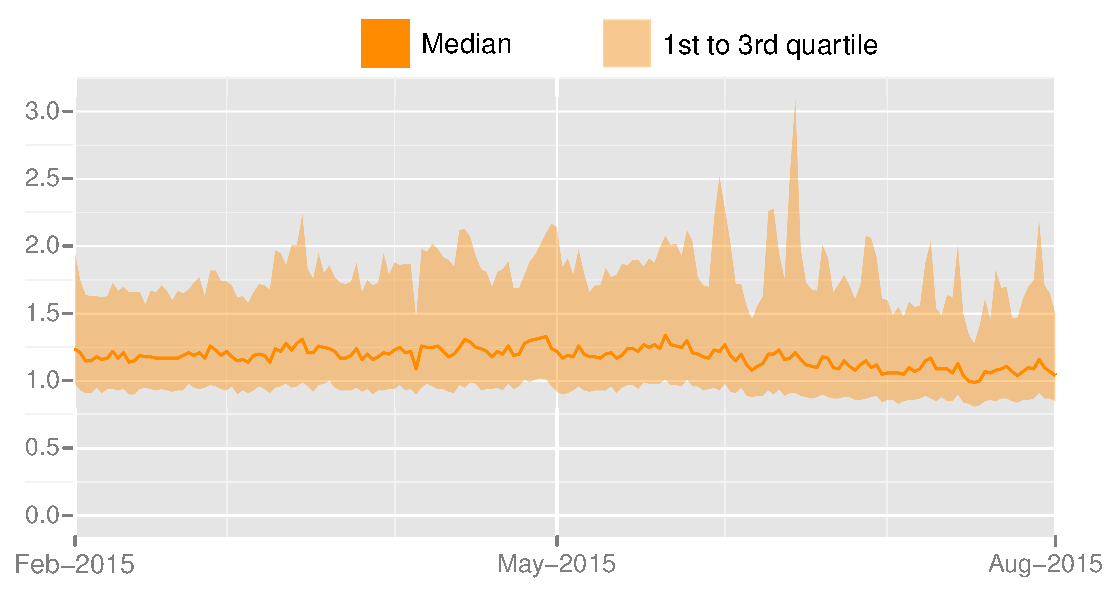
\includegraphics[width=\linewidth]{../assets/images/torperf_50kb_2015-02_2015-08.eps}
	\caption{The average performance to download 50 KB files over Tor circuits, as measured by Tor bandwidth authorities. The first and third quartiles are shown with the median time shown in orange \cite{TorMetrics}.}
	\label{fig:latencyGraph}
\end{figure}

This network latency to query a OnioNS Mirror is supplemental to the time to verify the Record and Merkle subtree. We avoid additional latency costs by implementing a client-side cache in order to allow subsequent queries to be resolved locally. We also reduce the expense of circuit construction by building the circuit on startup.

\subsubsection{Usability}

Our software maximizes usability in for two main groups of users: hidden service administrators and Tor end-users. The OnioNS-HS command-line utility provides minimal prompts: it asks the user for the main domain name, a list of subdomains and destinations, and the user's PGP key if they choose to disclose it. It then loads the hidden service private key, performs the proof-of-work to validate the Record, and automatically uploads the Record to the Quorum. We released a beta test of our software to Tor developers and volunteers and received positive feedback on the simplicity of the registration process.

Our client software integrates well into the Tor Browser and starts and stops with the Tor Browser environment. As shown in Figure \ref{fig:prototypeExample}, OnioNS resolves and loads hidden services under a meaningful name transparently without requiring any user interaction, similar to traditional DNS requests over Tor circuits. We observed that queries for unknown domains added several seconds of latency to the load time of hidden services, matching our above analysis. Similar to the BIND software for DNS, OnioNS-client caches known Records in local storage, allowing further queries for their domains to be resolved nearly instantaneously. This mechanism also accelerates load times if those Records are part of a chain of resolutions. Local resolution also minimizes a Mirror's exposure to the popularity of domain names.

%We also maintain significant usability and security benefits over similar systems such as Namecoin. OnioNS Records 

We achieve another primary usability benefit by introducing an automatic naming system for Tor hidden services: it is no longer necessary for the Tor community to construct and maintain directories of hidden services. The automatic resolution of domain names allows scaling beyond human-maintained directories, which only efficiently scales to several hundred names at most. OnioNS should provide a significant usability to Tor users and the community at large.

\subsection{Discussions}

In this section we further discuss and compare our work with related works. The Onion Name System and Namecoin both achieve all three properties of Zooko's Triangle, and while the two systems share some design similarities, each system is constructed with different threat models and different objectives in mind.

Namecoin's security rests on two primary assumptions: that its network is resistant to Sybil attacks and that more than 50 percent of the network's computational power is at least semi-honest. An attacker who gained the majority of the computational power (a ``51\% attack'') may double-spend transactions, prevent new transactions from entering the honest blockchain, and prevent honest miners from contributing blocks. A successful Sybil attack on Namecoin's network allows an attacker to disrupt the network by purposefully not relaying blocks or transactions, providing attacker-controlled data to clients, or by increasing the potential for double-spending attacks. Namecoin's blockchain has an indefinite length in order to allow the network to trace transactions and ownership of Namecoins back to their originating source. It relies on each participant in the Namecoin network to hold, validate, and read from its own local copy of the blockchain. The CPU, bandwidth, and memory requirements for anyone holding the blockchain scales linearly as the age and popularity of the Namecoin system increases.

By contrast, OnioNS' central security assumption is that circuits through the Tor network provide privacy. This assumption implies that the Tor network remains resistant to Sybil attack, traffic analysis, and that the majority of the directory authorities remain semi-honest. We have shown that a sufficiently-large Quorum remains strongly resistant to large-scale Sybil attacks on the Tor network. Thus, we do not introduce a new network for our naming system and instead utilize the Tor network to achieve both communication privacy and the infrastructure for OnioNS. If an attacker gains control of the Tor network (such as by Sybil attack or by compromising the directory authorities) then circuits no longer provide privacy, hidden services can be de-anonymized, and a privacy-enhanced naming system no longer becomes necessary. We do not also rely on assumptions of computational power: unlike Namecoin, attackers with large computational capacities are not able to disrupt network communication or to provide malicious responses to client queries.

Both Namecoin and OnioNS utilize append-only data structures for long-term storage. Namecoin typically requires clients to either hold their own copy of the blockchain, rely on the honesty of their Namecoin-compatible DNS server, or to utilize a Simplified Payment Verification \cite{nakamoto2008bitcoin} (SPV) scheme which allows clients to download and verify minimalistic information from a central server. These latter two cases are vulnerable to a variety of attacks if the server is malicious and neither approach provides authenticated denial-of-existence. OnioNS does also not require clients to download the Pagechain; instead, clients receive a minimal number of mappings, a Merkle subtree, and Quorum signatures on the root hash. Our protocols prevent a malicious server from acting dishonestly, including spoofing mappings or falsely claiming non-existence. The security of the response depends on our security assumptions regarding the Quorum.

Namecoin and OnioNS allow full enumeration of all registered domains; name registrations are assumed to be public knowledge immediately after they are uploaded to either network. We do not consider this a significant threat to our system as registrations do not contain personal information. Similar to Namecoin, anyone may obtain a complete copy of the Pagechain and Mirrors must be able to access and verify all information in the Pagechain in order to respond to client queries.

Both OnioNS and Namecoin operate under weaker adversarial models than the GNU Name System. GNS assumes than attacker may participant in any role, may infiltrate the network by large-scale Sybil attack, and is assumed to have more computational power than all honest participants combined. Neither Namecoin, OnioNS, nor Tor provide full defences against such well-resourced adversaries. Tor hidden services may become de-anonymized under GNS' adversarial model so we do not assume that our adversaries are that powerful. End-users should select their naming system carefully according to their threat model.

\section{Conclusions and Future Work}

We have presented the Onion Name System (OnioNS), a distributed, secure, and usable alternative DNS that maps globally-unique and meaningful .tor domains to .onion hidden service addresses, and achieve all three properties of Zooko's Triangle. We enable any hidden service operator to anonymously claim a human-readable name for their server and clients to query the system in privacy-enhanced manner. We introduce a distributed blockchain-based database and mechanisms that let clients authenticate and verify denial-of-existence claims. Additionally, we utilize the existing and semi-trusted infrastructure of Tor, which significantly narrows our threat model to already well-understood attack surfaces and allows our system to be integrated into Tor with minimal effort. Our reference implementation demonstrates high usability and shows that OnioNS successfully addresses the major usability issue that has been with Tor hidden services since their introduction in 2002.

In future work we will expand our implementation and pursuit integrating it into Tor. OnioNS requires a few changes to Tor, namely a new .tor pseudo-TLD and Ed25519 router keys, but we introduce no changes to Tor's hidden service protocol. Should Tor's developers introduce changes to the hidden service protocol, OnioNS can become forwards-compatible with a few changes. Additionally, our implementation currently only supports ASCII characters in domain names, so in future work we will explore implementing Punycode to provide support for international character sets. Unlike the Internet DNS, we will disallow digits zero and one (similar to base32 encoding) in order to reduce the threat of phishing attacks from spoofed domains with indistinguishable characters.

%
%\section*{Acknowledgements}
%
%We would like to thank Roger Dingledine, George Kadianakis, Yawning Angel, and Nick Mathewson for their support, commentary, and assistance with Tor technical support.
%
%%We would like to thank Tor developers and volunteers within the community for technical support and their commentary on our work.
%
%\newpage
%
%
%
%
%
%
%%, a password-based key derivation function which is notable for its large memory and CPU requirements during its operation. The scrypt function provides significantly greater resistance to custom hardware attacks and massively parallel computation primarily due to its memory requirements. This limits attackers to the same software implementation and asymptotic cost as legitimate users\cite{percival2009stronger}\cite{percival2012scrypt}. We choose scrypt because of these advantages over other key derivation functions such as SHA-256 or PBKDF2. For these reasons scrypt is also common for proof-of-work purposes in some cryptocurrencies such as Litecoin.
%
%% ----------------------------------------------------------------------------------------
%
%% An example of a floating figure using the graphicx package.
%% Note that \label must occur AFTER (or within) \caption.
%% For figures, \caption should occur after the \includegraphics.
%% Note that IEEEtran v1.7 and later has special internal code that
%% is designed to preserve the operation of \label within \caption
%% even when the captionsoff option is in effect. However, because
%% of issues like this, it may be the safest practice to put all your
%% \label just after \caption rather than within \caption{}.
%%
%% Reminder: the "draftcls" or "draftclsnofoot", not "draft", class
%% option should be used if it is desired that the figures are to be
%% displayed while in draft mode.
%%
%%\begin{figure}[!t]
%%\centering
%%\includegraphics[width=2.5in]{myfigure}
%% where an .eps filename suffix will be assumed under latex, 
%% and a .pdf suffix will be assumed for pdflatex; or what has been declared
%% via \DeclareGraphicsExtensions.
%%\caption{Simulation Results}
%%\label{fig_sim}
%%\end{figure}
%
%% Note that IEEE typically puts floats only at the top, even when this
%% results in a large percentage of a column being occupied by floats.
%
%% ----------------------------------------------------------------------------------------
%
%% An example of a double column floating figure using two subfigures.
%% (The subfig.sty package must be loaded for this to work.)
%% The subfigure \label commands are set within each subfloat command, the
%% \label for the overall figure must come after \caption.
%% \hfil must be used as a separator to get equal spacing.
%% The subfigure.sty package works much the same way, except \subfigure is
%% used instead of \subfloat.
%%
%%\begin{figure*}[!t]
%%\centerline{\subfloat[Case I]\includegraphics[width=2.5in]{subfigcase1}%
%%\label{fig_first_case}}
%%\hfil
%%\subfloat[Case II]{\includegraphics[width=2.5in]{subfigcase2}%
%%\label{fig_second_case}}}
%%\caption{Simulation results}
%%\label{fig_sim}
%%\end{figure*}
%%
%% Note that often IEEE papers with subfigures do not employ subfigure
%% captions (using the optional argument to \subfloat), but instead will
%% reference/describe all of them (a), (b), etc., within the main caption.
%
%% ----------------------------------------------------------------------------------------
%
%% An example of a floating table. Note that, for IEEE style tables, the 
%% \caption command should come BEFORE the table. Table text will default to
%% \footnotesize as IEEE normally uses this smaller font for tables.
%% The \label must come after \caption as always.
%%
%%\begin{table}[!t]
%%% increase table row spacing, adjust to taste
%%\renewcommand{\arraystretch}{1.3}
%% if using array.sty, it might be a good idea to tweak the value of
%% \extrarowheight as needed to properly center the text within the cells
%%\caption{An Example of a Table}
%%\label{table_example}
%%\centering
%%% Some packages, such as MDW tools, offer better commands for making tables
%%% than the plain LaTeX2e tabular which is used here.
%%\begin{tabular}{|c||c|}
%%\hline
%%One & Two\\
%%\hline
%%Three & Four\\
%%\hline
%%\end{tabular}
%%\end{table}
%
%% ----------------------------------------------------------------------------------------
%
%% Note that IEEE does not put floats in the very first column - or typically
%% anywhere on the first page for that matter. Also, in-text middle ("here")
%% positioning is not used. Most IEEE journals/conferences use top floats
%% exclusively. Note that, LaTeX2e, unlike IEEE journals/conferences, places
%% footnotes above bottom floats. This can be corrected via the \fnbelowfloat
%% command of the stfloats package.
%
%% conference papers do not normally have an appendix
%
%% ----------------------------------------------------------------------------------------
%
%% trigger a \newpage just before the given reference
%% number - used to balance the columns on the last page
%% adjust value as needed - may need to be readjusted if
%% the document is modified later
%%\IEEEtriggeratref{8}
%% The "triggered" command can be changed if desired:
%%\IEEEtriggercmd{\enlargethispage{-5in}}
%
%% references section can use a bibliography generated by BibTeX as a .bbl file
%% BibTeX documentation can be easily obtained at:
%% http://www.ctan.org/tex-archive/biblio/bibtex/contrib/doc/
%% The IEEEtran BibTeX style support page is at:
%% http://www.michaelshell.org/tex/ieeetran/bibtex/
%%\bibliographystyle{IEEEtranS}
%% argument is your BibTeX string definitions and bibliography database(s)
%%\bibliography{IEEEabrv,../bib/paper}
%%
%% <OR> manually copy in the resultant .bbl file
%% set second argument of \begin to the number of references
%% (used to reserve space for the reference number labels box)
%%\begin{thebibliography}{1}
%%
%%\bibitem{IEEEhowto:kopka}
%%H.~Kopka and P.~W. Daly, \emph{A Guide to \LaTeX}, 3rd~ed.\hskip 1em plus
%%  0.5em minus 0.4em\relax Harlow, England: Addison-Wesley, 1999.
%%
%%\end{thebibliography}
%
\bibliographystyle{abbrv}
\bibliography{citations}

% that's all folks
\end{document}
